%****************************************************
%	CHAPTER 3 - THEORETICAL DEVELOPMENT
%****************************************************
\chapter{Theoretical Background}
\label{chap:theory}
In order to understand the \ac{hh} inversion technique, the theoretical foundations surrounding the modelling of ocean waves, in both deep and shallow water, need to be understood. Furthermore, a foundational understanding of \ac{sar}, encompassing its data acquisition and types, along with the pre-processing techniques applied in implementing the \ac{hh} technique to achieve the desired outcomes, is necessary.

This chapter's objective is to introduce the theoretical aspects surrounding these fields, thereby providing context for the subsequent chapter's introduction of the pipeline design. Additionally, this chapter builds upon the theories previously discussed in Chapter \ref{chap:litReview}. In this chapter, key terms are useful to enhance the understanding of the reader. Field-specific terms are briefly introduced in the \nameref{chap:glossary} and provide context to the terms used in the subsequent sections.

%====================================================
% OCEAN WAVES
%====================================================
\section{Ocean Waves} \label{sec:theory.waves}
The majority of this section draws upon content collated by Holthuijsen \cite{Holthuijsen2007}, with equations and figures cited appropriately. The objective of this section is to provide an introductory overview of the fundamental theory related to ocean waves and their mathematical modelling as well as highlighting the differences in this modelling in deep and shallow water. Appropriate, and relevant derivations and visual explanations of key concepts are included in Appendix \ref{ap:oceanWaves}. %Furthermore, the way in which waves are attenuated and dispersed upon entering the \ac{miz} in Antarctica is discussed.

\subsection{Description of Ocean Waves} \label{subsec:theory.waves.description}

The wave height, $H$, can be defined as the vertical distance between the lowest and highest surface elevation in a wave. Where surface elevation, denoted using $\eta(t)$, refers to the instantaneous elevation of the sea surface relative to some reference level. The zero-crossing wave period, $T_{0}$, can be defined as the time between one zero-down crossing and the following one. Where a zero-down crossing is the crossing of the mean surface elevation when the gradient of the wave is negative. All of these terms are depicted in Figure \ref{fig:theory.waves.introFigure}.

\begin{figure}[H]
    \centering
    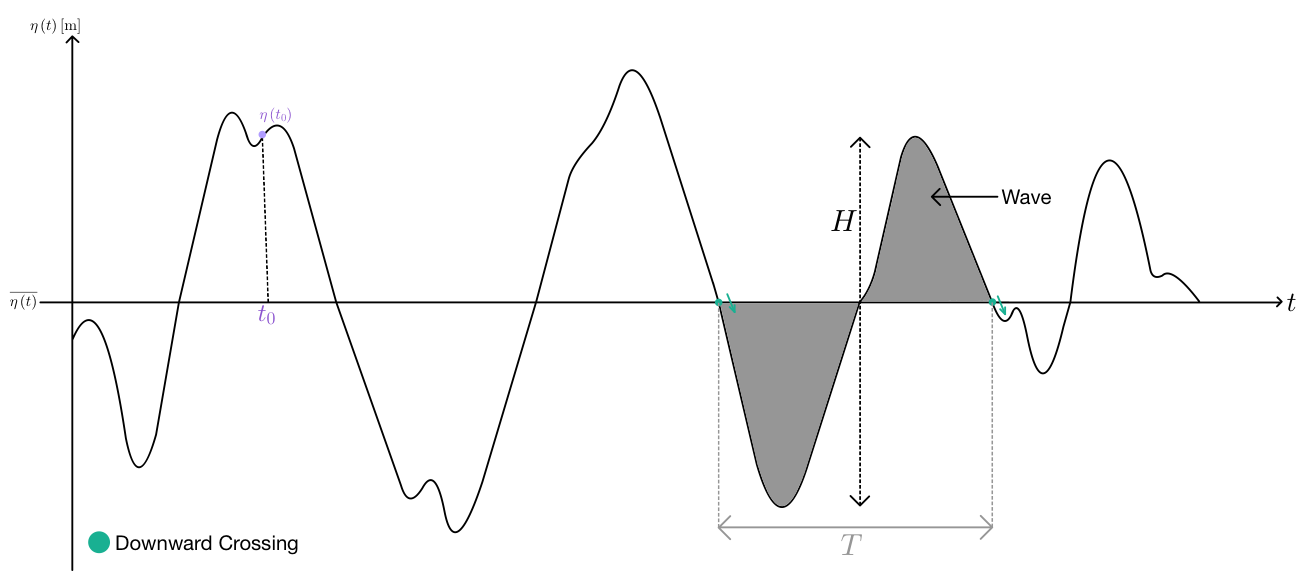
\includegraphics[width=.8\linewidth]{Figures/Theory/placeholder_waveDefinitions.png}
    \caption{Visual definition of surface elevation ($\eta(t)$), wave height ($H$), wave period ($T$), and zero-down crossing. Adapted from \cite{Holthuijsen2007}.}
    \label{fig:theory.waves.introFigure}
\end{figure}

Holthuijsen \cite{Holthuijsen2007} defines the following equations for the mean wave height and zero-crossing wave period for $N$ wave where $i$ represents the sequence number of the waves in the \gls{waveRecord}.

\begin{equation} \label{eq:waves.mean(H)}
    \overline{H} = \frac{1}{N}\sum_{i}^{N}H_{i}
\end{equation}

\begin{equation} \label{eq:waves.mean(T0)}
    \overline{T_{0}} = \frac{1}{N}\sum_{i}^{N}T_{0,i}
\end{equation}

The definition of the significant wave height and wave period follows, where $j$ is the rank number of the sequence of waves, based on wave height, in descending order. The significant wave height is a useful metric, as it can be estimated from the wave spectrum \cite{Holthuijsen2007}, which is introduced in the subsequent subsection.

\begin{equation} \label{eq:waves.sigH}
    H_{1/3} = \frac{1}{N/3}\sum_{j}^{N/3}H_{j}
\end{equation}

\begin{equation} \label{eq:waves.sigT}
    T_{1/3} = \frac{1}{N/3}\sum_{j}^{N/3}T_{0,j}
\end{equation}

\subsection{Wave Spectra} \label{subsec:theory.waves.waveSpectrum}
Include info about stationary measurements
\subsubsection{Random Phase/Amplitude Model} \label{subsec:theory.waves.waveSpectrum.randModel}

The wave spectrum aims to describe the ocean surface as a stationary stochastic process\footnote{define stochastic process}. It is based on the random-phase/amplitude model, where the surface elevation is treated as the sum of a large number of harmonic waves. Each of these waves possesses a constant amplitude and a phase that is randomly selected for each time record realisation. This approach enables the modelling of the wave spectrum as a Fourier series, as illustrated in Equation \ref{eq:waveSpectrum.fourierSeries}. For a more detailed explanation, please refer to Appendix \ref{sec:ap.oceanWaves.randModel}.

\begin{equation} \label{eq:waveSpectrum.fourierSeries}
    \underline{\eta}(t) = \sum_{i=1}^{N}\underline{a}_{i}cos(2\pi f_{i}t + \underline{\phi}_{i})
\end{equation}

ADD NOTES ON APPLICABILITY OF RANDOM MODEL (pg. 35 - beginning 36)

\subsubsection{Variance Density Spectrum} \label{subsec:theory.waves.waveSpectrum.varianceSpectrum}

The variance density spectrum can be constructed by utilising the variance, $E\left \{  \frac{1}{2}\underline{a}^{2}_{i}\right \}$, as opposed to the expected value, $E\left \{  \underline{a}_{i}\right \}$. [Use note 3A to explain variance] Also explain why variance is better than using expected value [variance is chosen as it allows the change over different samples to be seen, as opposed to the pure magnitude.]
% This choice to use variance is preferred as it allows changes across different samples to be observed, rather than each sample's pure magnitude.

In order to mitigate the second issue with the application of the random phase/amplitude model, it is modified by distributing the variance over the frequency interval $\Delta f_{i}$ and the frequency $f_{i}$. This gives rise to the variance \textbf{density} spectrum, $E^{*}\left \{ \frac{1}{2}  \underline{a}^{2}_{i}\right \}$.


\begin{equation} \label{eq:waveSpectrum.varianceDSpectrum}
    E^{*}\left \{  f_{i}\right \} = \frac{1}{\Delta f_{i}}E\left \{\frac{1}{2}  \underline{a}^{2}_{i}\right \} \; \; \; \text{for all} \; \; \;  f_{i}
\end{equation}

Whilst Equation \ref{eq:waveSpectrum.varianceDSpectrum} is defined for all frequencies, it is still discontinuous between frequency bands. A continuous version of $E^{*}\left \{  f_{i}\right \}$ can be determined by taking the limit as $\Delta f_{i}$ tends to zero. This entire process is graphically depicted in Figure \ref{fig:theory.waves.waveSpectrum.varianceDSpectrum}.

\begin{equation} \label{eq:waveSpectrum.varianceDSpectrumCont}
    E(f) = \lim_{\Delta f \to 0}\frac{1}{\Delta f}E\left \{ \frac{1}{2} \underline{a}^{2}\right \}
\end{equation}
[Show graphically with FIG 3.7 - pg. 37]

\begin{figure}[H]
    \centering
    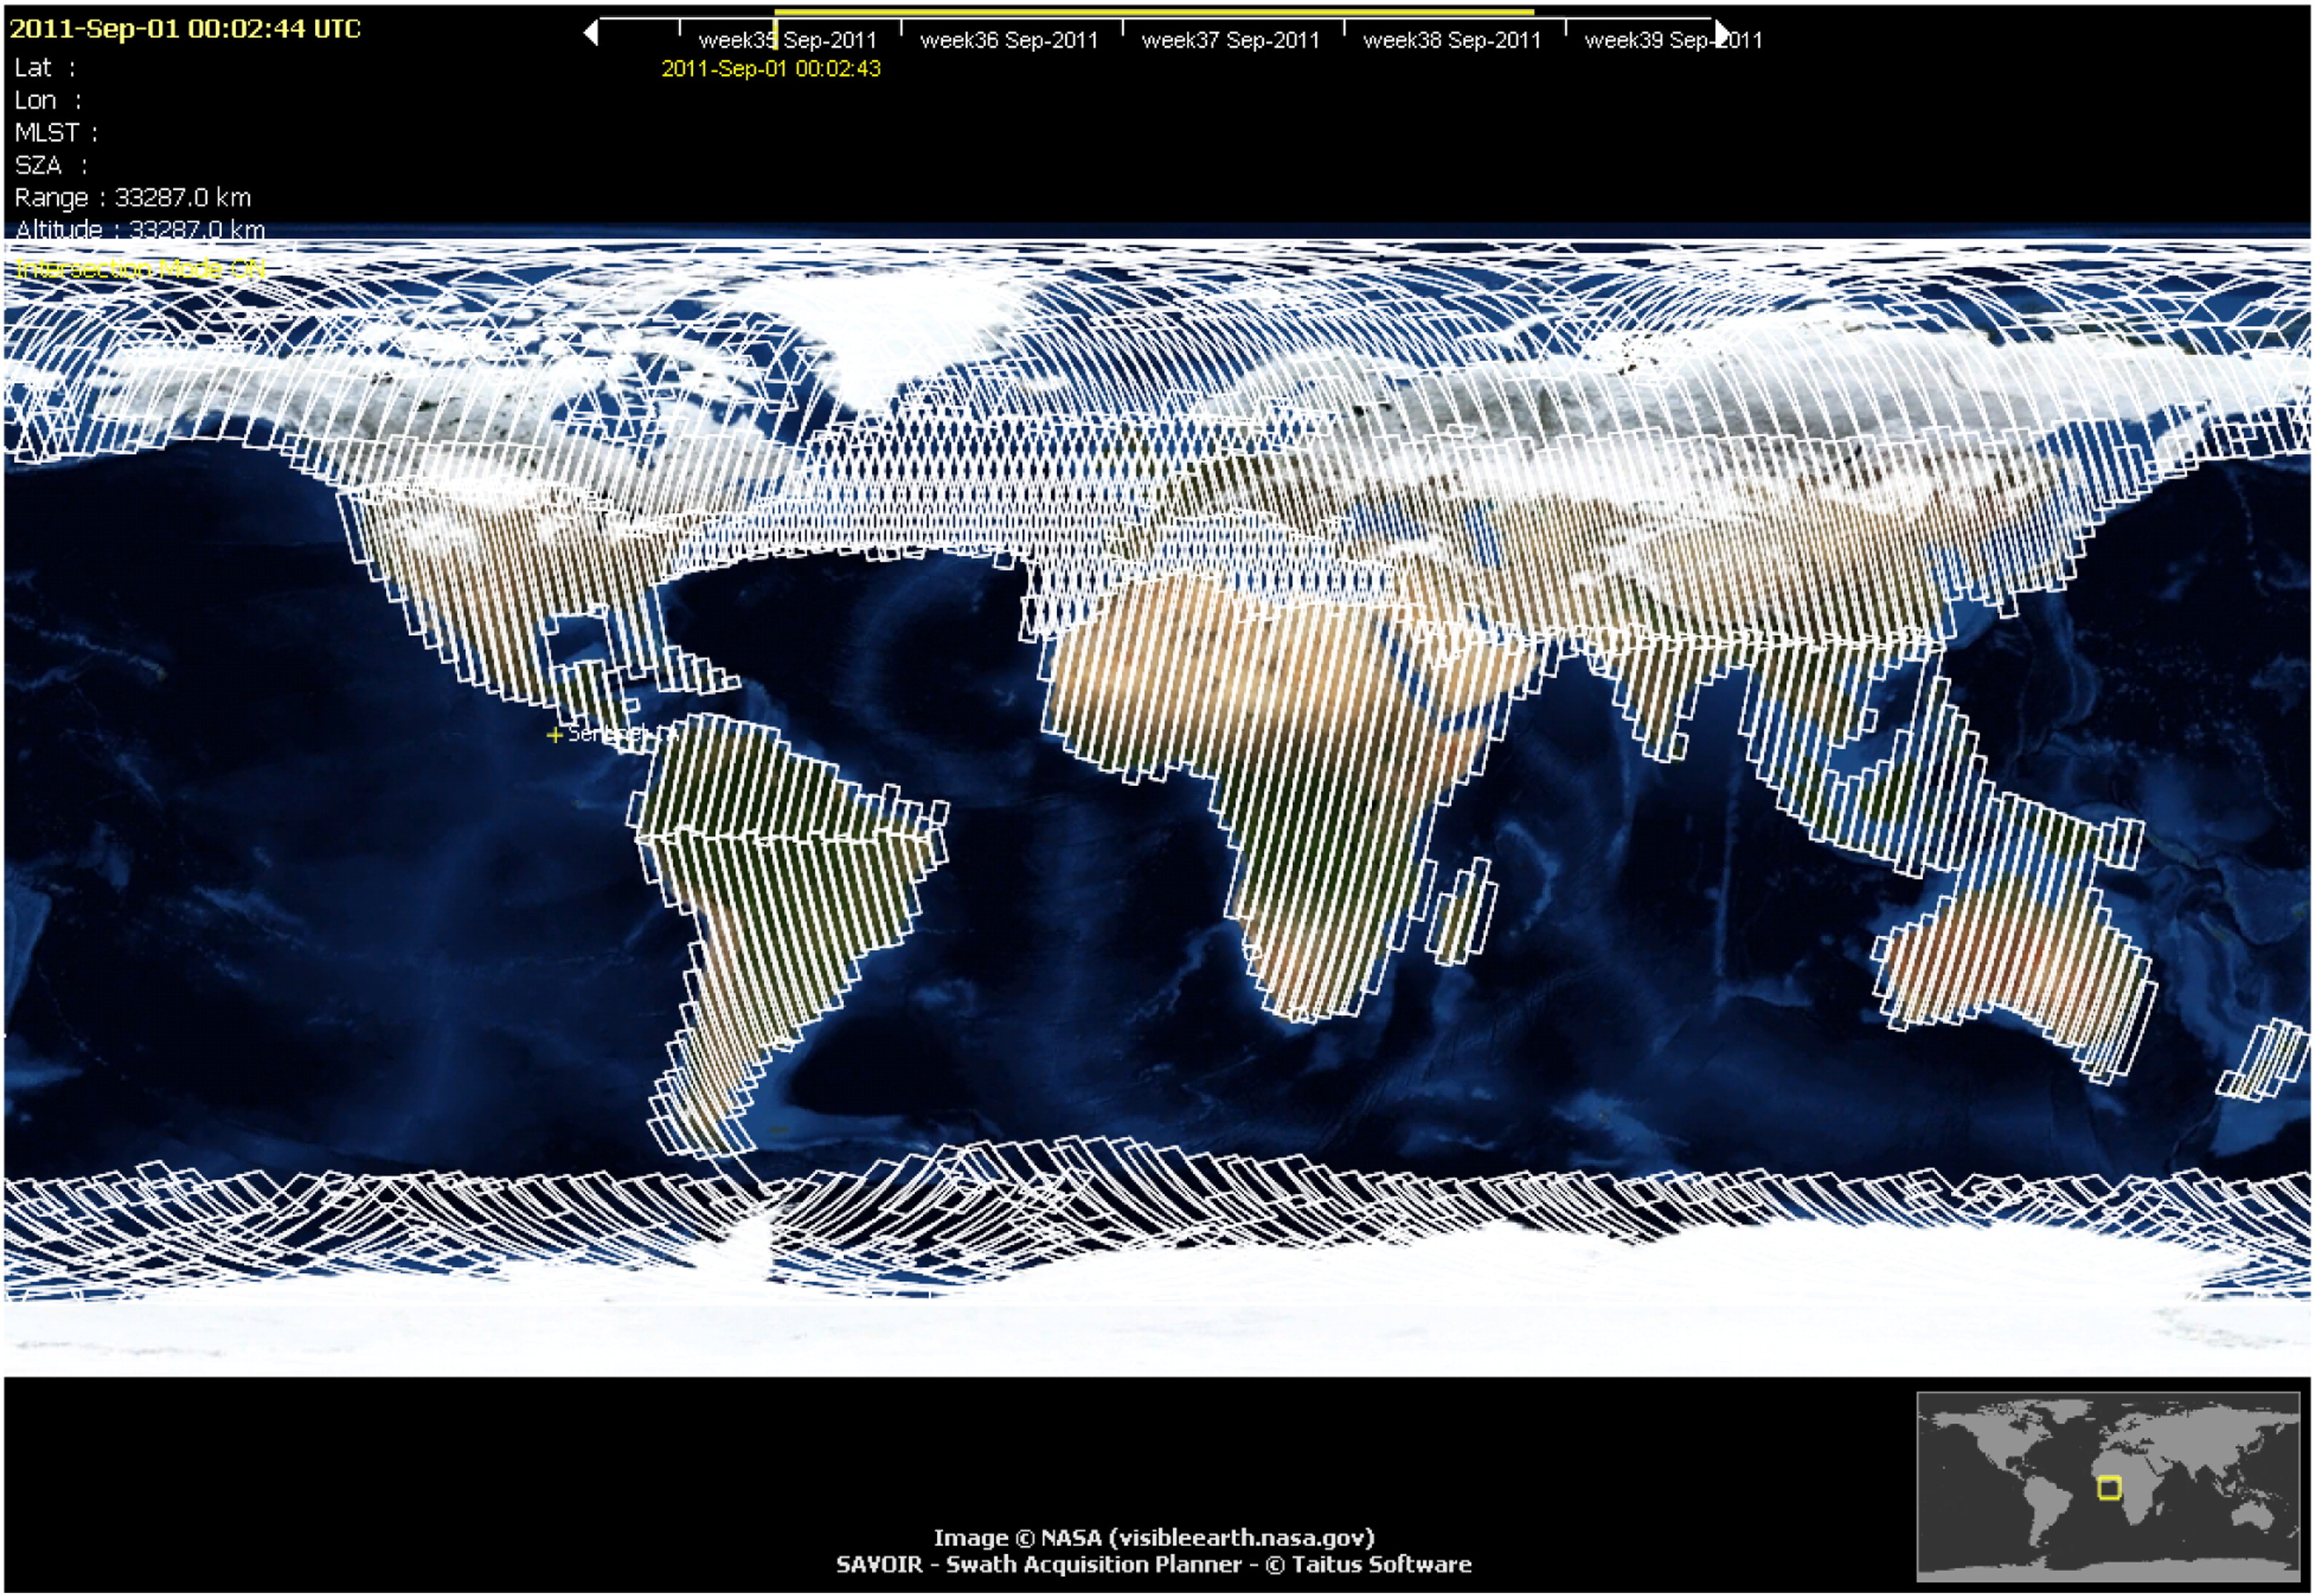
\includegraphics[width=.5\linewidth]{Figures/LiteratureReview/Satellites/sentinelCoverage.jpg}
    \caption{Visual explanation of the transformation from discrete amplitude spectrum of the random phase/amplitude model (top frame), depicted in Figure \ref{fig:ap.randModel}, to the continuous variance density spectrum (bottom frame). Adapted from \cite{Holthuijsen2007}.}
    \label{fig:theory.waves.waveSpectrum.varianceDSpectrum}
\end{figure}

The variance density spectrum provides a complete description of the surface elevation of ocean waves as all statistical characteristics of the wave field can be expressed in terms of this spectrum, provided it is modelled as a stationary, Gaussian process.

% The units of the variance density spectrum, $E(f)$, can be derived as follows.
% \begin{gather*}
%     \frac{1}{\Delta f}E\left \{ \frac{1}{2} \underline{a}^{2}\right \} \; \; \; \text{has units:}\\
%     \frac{1}{\text{s}^{-1}}\text{m}^{2} = \text{m}^{2}\text{s} = \text{m}^{2}/\text{Hz}
% \end{gather*}

% The allows the total variance, $\overline{\underline{\eta}^{2}}$, to be calculated as follows.

% \begin{equation} \label{eq:waveSpectrum.totalVar}
%     \overline{\underline{\eta}^{2}} = \int_{0}^{\infty} E(f)df
% \end{equation}


\subsubsection{Spectral Domain Definition} \label{subsec:theory.waves.waveSpectrum.spectralDef}
Equations \ref{eq:waveSpectrum.fourierSeries},\ref{eq:waveSpectrum.varianceDSpectrumCont} are defined in terms of time and frequency. In order to represent the variance density spectrum in the radian frequency, $\omega$, the relationship, $\omega = 2\pi/T$ needs to be used. Equation \ref{eq:waveSpectrum.fourierSeries} is then updated to the following form

\begin{equation} \label{eq:waveSpectrum.fourierSeries_omega}
    \underline{\eta}(t) = \sum_{i=1}^{N}\underline{a}_{i}cos(\omega t + \underline{\phi}_{i})
\end{equation}

This allows the variance density spectrum, $E(\omega)$, to be defined as follows, where $J$ represents the Jacobian. In this case, $J=1/2\pi$.
\begin{equation} \label{eq:waveSpectrum.relateE(f)toE(w)}
    E(\omega) =  E(f) \frac{df}{d\omega} = E(f)J = \frac{1}{2\pi}E(f)
\end{equation}

\subsubsection{Frequency-direction Spectrum} \label{subsec:theory.waves.waveSpectrum.freqDirection}
The variance density spectrum equation as described in Equation \ref{eq:waveSpectrum.varianceDSpectrumCont} represents a one-dimensional function of time. In order to consider a two-dimensional spectrum, the random phase/amplitude model needs to be expanded to consider a wave propagating in the $x,y$-space in a direction $\theta$, relative to the +$x$-axis. This allows the model to be expanded as follows, where the wave number, $k = 2\pi/L$ with $L$ equal to the length of the harmonic wave.

\begin{equation} \label{eq:waveSpectrum.fourierSeries_3D}
    \underline{\eta}(x,y,t) = \sum_{i=1}^{N} \sum_{j=1}^{M} \underline{a}_{i,j}cos(\omega_{i}t-k_{i}xcos(\theta_{j}) - k_{i}ysin(\theta_{j}) + \underline{\phi}_{i,j})
\end{equation}

where each wave component is indicated by two indices.
\begin{itemize}
    \item $i$: The frequency index or wave number
    \item $j$: The direction
\end{itemize}

Following the same process of transforming a one-dimensional amplitude spectrum into a continuous variance density spectrum, as detailed in Equations \ref{eq:waveSpectrum.varianceDSpectrum}, \ref{eq:waveSpectrum.varianceDSpectrumCont}, the two-dimensional variance density spectrum is found as

\begin{equation} \label{eq:waveSpectrum.varianceDSpectrumCont_2D}
    E(\omega,\theta) =  \lim_{\Delta \omega \to 0}\lim_{\Delta \theta \to 0}\frac{1}{\Delta \omega \Delta \theta} E\left \{ \frac{1}{2} \underline{a}^{2}\right \}
\end{equation}

Using the Jacobian determined in Equation \ref{eq:waveSpectrum.relateE(f)toE(w)}, the same relationship can be developed for the two-dimensional variance density spectrum

\begin{equation} \label{eq:waveSpectrum.relateE(f)toE(w)_2D}
    E(\omega,\theta) =  \frac{1}{2\pi}E(f,\theta)
\end{equation}

\subsection{Wave-number Spectra} \label{subsec:theory.waves.waveNumberSpectra}
Where the wave spectrum considers the sea as a function of space and time, $\eta(x,y,t)$, the ocean can also be considered as a function of space at a single moment in time. This idea is useful for remote sensing applications.

% \subsubsection{One-dimensional spectrum} \label{subsec:theory.waves.waveNumberSpectra.1D}
% The definition of the one-dimensional wave-number spectrum is identical to the frequency-direction spectrum, however, the time is replaced by the horizontal coordinate, $x$, and the radian frequency is replaced by the wave number, $k$. This allows $E(k)$ to be defined as the following, where $\Delta k$ is the wave-number bandwidth.

% \begin{equation} \label{eq:waveNumberSpectrum.E(K)_1D}
%     E(k) = \lim_{\Delta k \to 0} \frac{1}{\Delta k} E\left \{ \frac{1}{2} \underline{a}^{2}\right \}
% \end{equation}

% In order to transform the wave-number spectrum into the frequency spectrum the following formula can be used. The Jacobian is found to be $c_{g}$, the velocity at which the waves propagate.

% \begin{equation} \label{eq:waveNumberSpectrum.relateE(f)toE(w)_1D}
%     E(k) =  E(\omega) \frac{d\omega}{dk} = c_{g}E(\omega)
% \end{equation}

\subsubsection{Two-dimensional spectrum} \label{subsec:theory.waves.waveNumberSpectra.2D}
In order to define the two-dimensional wave-number spectrum, the method described in Equations \ref{eq:waveSpectrum.fourierSeries}, \ref{eq:waveSpectrum.varianceDSpectrumCont} can be used. Where $\Delta k_{x}$ and $\Delta k_{y}$ represent the spectral bandwidths.

\begin{equation} \label{eq:waveNumberSpectrum.fourierSeries_2D}
    \eta(x,y) = a_{i,j}cos(k_{x,i}x + k_{y,j}y + \phi_{i,j})
\end{equation}

\begin{equation} \label{eq:waveNumberSpectrum.SpectrumCont_2D}
    E(k_{x},k_{y}) = \lim_{\Delta k_{x} \to 0} \lim_{\Delta k_{y} \to 0} \frac{1}{\Delta k_{x} \Delta k_{y}} E\left \{ \frac{1}{2} \underline{a}^{2}\right \}
\end{equation}

With $k_{x} = k\cos(\theta)$, and $k_{y} = k\sin(\theta)$, $k$ and $\theta$ can be defined as: $k = \sqrt{k_{x}^2 + k_{y}^2}$ and $\theta = \text{arctan}(k_{y}/k_{x})$. This allows an equivalent spectrum to be defined in terms of $k$ and $\theta$.

\begin{equation} \label{eq:waveNumberSpectrum.SpectrumCont_2D_kTh}
    E(k,\theta) = \lim_{\Delta k \to 0} \lim_{\Delta \theta \to 0} \frac{1}{\Delta k \Delta \theta} E\left \{ \frac{1}{2} \underline{a}^{2}\right \}
\end{equation}

These two spectra are related by the following relationship.
\begin{equation} \label{eq:waveNumberSpectrum.relateE(k,th)toE(kx,ky)_2D}
    E(k,\theta) =  E(k_{x},k_{y}) J = k E(k_{x},k_{y})
\end{equation}

The two-dimensional frequency-direction spectrum in Equation \ref{eq:waveSpectrum.varianceDSpectrumCont_2D} is related to the spectrum in Equation \ref{eq:waveNumberSpectrum.SpectrumCont_2D} by the following relationship, where $c_{w} = \omega /k$ and the Jacobian, $J = 1/c_{g}$. $c_{w}$ and $c_{g}$ are defined as the wave speed and group wave speed respectively and are discussed in the following subsection.
\begin{equation} \label{eq:waveNumberSpectrum.relateE(kx,ky)toE(w,th)_2D}
    E(k_{x},k_{y}) =  k E(\omega,\theta) J = \frac{c_{w} c_{g}}{\omega} E(\omega,\theta)
\end{equation}

These two-dimensional spectra are useful in two different applications, however, in varying forms.
\begin{itemize}
    \item Remote sensing: $E(k_{x},k_{y})$
    \item Wave models: $E(f,\theta)$
\end{itemize}

\subsection{Linear Wave Theory} \label{subsec:theory.waves.linearWaveTheory}

The linear theory for \gls{oceanWaves} provides a detailed description of harmonic waves. It relies on two equations and associated boundary conditions, which are discussed in Chapter 5.3 of \cite{Holthuijsen2007}. The solution to the kinematic boundary conditions results in a wave propagating in the $x$-direction. This propagating harmonic can be described in two different ways.

\begin{subequations}  \label{eq:linearWaveTheory.propHarmonicWave}
  \begin{align}
    \eta(x,t) = a\text{sin}(\omega t - kx) \\
    \eta(x,t) = \frac{H}{2}\text{sin} \left ( \frac{2\pi}{T}t - \frac{2\pi}{L}x \right )
  \end{align}
\end{subequations} 


\begin{itemize}
    \item Illustration on page 119
\end{itemize}

% Include derivation of c_wave - page 119

\subsection{Ocean Wave Dynamics} \label{subsec:theory.waves.dynamics}

Considering the harmonic surface profile of ocean waves, as well as the velocity potential function, which are described by Holthuijsen in Chapter 5.4.2 \cite{Holthuijsen2007}, a relationship, known as the dispersion relationship can be developed.

\subsubsection{Dispersion Relationship} \label{subsec:theory.waves.dynamics.dispersionRelationship}

The dispersion relationship relates the radian frequency, $\omega$, to the wave number, $k$ \cite{Holthuijsen2007}. The dispersion relationship for an arbitrary depth is given as 

\begin{equation} \label{eq:linearWaveTheory.dispersionRelationship}
    \omega ^2 = gk\text{tanh}(kd).
\end{equation}

The propagation speed of a wave can be determined from Equation \ref{eq:linearWaveTheory.dispersionRelationship} with the fact that $c_{w} = \omega / k$. This gives the wave phase speed for an arbitrary depth as

\begin{equation} \label{eq:linearWaveTheory.phaseVelocity}
    c_{w} = \frac{g}{\omega}\text{tanh}(kd) = \sqrt{\frac{g}{k}\text{tanh}(kd)}
\end{equation}

Considering Equation \ref{eq:linearWaveTheory.dispersionRelationship} and \ref{eq:linearWaveTheory.phaseVelocity} for both deep water and shallow water yields the following approximations to be determined.

\subsubsection{Deep Water} \label{subsec:theory.waves.linearWaveTheory.deepWater}

In deep water, the term, $kd \to \infty$, and due to this, $\text{tanh}(kd) \to 1$ \cite{Holthuijsen2007}. This means that the dispersion relationship for deep water approaches

\begin{equation} \label{eq:linearWaveTheory.dispersionRelationship.deepWater}
    \omega_{0} = \sqrt{gk_{0}}
\end{equation}

where $k_0$ is the deep water wave number. The same logic with respect to $kd \to \infty$ applies to the phase velocity and means that the deep water phase velocity reduces to 

\begin{equation} \label{eq:linearWaveTheory.phaseVelocity.deepWater}
    c_{w_0} = \sqrt{\frac{g}{k_{0}}} = \frac{g}{\omega_{0}}  = \frac{g}{2\pi}T
\end{equation}

\subsubsection{Shallow Water} \label{subsec:theory.waves.linearWaveTheory.shallowWater}

In shallow water, the term, $kd \to 0$, and due to this, $\text{tanh}(kd) \to kd$ \cite{Holthuijsen2007}. This means that the dispersion relationship for shallow water approaches

\begin{equation} \label{eq:linearWaveTheory.dispersionRelationship.shallowWater}
    \omega = k\sqrt{gd}
\end{equation}

The same logic with respect to $kd \to 0$ applies to the phase velocity and means that the shallow water phase velocity reduces to 

\begin{equation} \label{eq:linearWaveTheory.phaseVelocity.shallowWater}
    c_{w_{shallow}} = \sqrt{gd}
\end{equation}

Equation \ref{eq:linearWaveTheory.phaseVelocity.shallowWater} shows that the phase speed does not depend on wavelength or frequency, and as such, this means that the waves are non-dispersive\footnote{non-dispersive defn.}.

\subsubsection{Adding Two Harmonic Waves} \label{subsec:theory.waves.linearWaveTheory.twoHarmonicWaves}

Using the definition of a propagating harmonic wave in Equation \ref{eq:linearWaveTheory.propHarmonicWave}, two of these waves can be combined in the following form.

\begin{equation} \label{eq:addingTwoWaves}
    \eta = \eta_{1} + \eta_{2} = a\text{sin}(\omega_{1}t - k_{1}x) + a\text{sin}(\omega_{2}t - k_{2}x)
\end{equation}

These two waves combine to create a sequence of wave groups. This group reaches its peak surface elevation when both $\eta_{1}$ and $\eta_{2}$ are in phase with each other. The phase velocity of these waves can be defined as the phase speed of the surface elevation envelope. This envelope can be determined by re-arranging Equation \ref{eq:addingTwoWaves} to give

% Fix with \left and \right
\begin{equation} \label{eq:addingTwoWaves.envelopeForm}
    \eta =  2a\text{cos} \left ( \frac{\omega_{1} - \omega_{2}}{2}t - \frac{k_{1} - k_{2}}{2}x \right ) \text{sin} \left ( \frac{\omega_{1} + \omega_{2}}{2}t - \frac{k_{1} + k_{2}}{2}x  \right )
\end{equation}

The cosine term acts as the envelope, while the sine term acts as the carrier wave \cite{Holthuijsen2007}. The phase velocity of the envelope represents the velocity of the wave group and can be derived as

\begin{equation} \label{eq:addingTwoWaves.envelopeVelocity}
    c_{envelope} = c_{g} = \frac{(\omega_{1} + \omega_{2})/2}{(k_1 + k_2)/2} = \frac{\Delta \omega}{\Delta k}
\end{equation}

As the frequencies and wave numbers can be considered as continuous, Equation \ref{eq:addingTwoWaves.envelopeVelocity} can be redefined as

\begin{equation} \label{eq:addingTwoWaves.groupVelocity}
    c_{g} = \frac{\partial \omega}{\partial k} = nc_{w}
\end{equation}

where $n$ is derived from Equation \ref{eq:linearWaveTheory.dispersionRelationship} as 

\begin{equation} \label{eq:addingTwoWaves.n}
    n = \frac{1}{2} \left ( 1+ \frac{2kd}{\text{sinh}(2kd)} \right )
\end{equation}

This value for $n$ varies between $\frac{1}{2}$ for deep water ($kd \to \infty$), and 1 for shallow water \cite{Holthuijsen2007} ($kd \to 0$) and implies that $c_{w} \geq c_{g}$. 

\subsection{Wave Modelling for Idealised Cases} \label{subsec:theory.waves.modelling}

\subsubsection{One-dimensional Wave Spectrum} \label{subsubsec:theory.waves.modelling.1D}

The one-dimensional wave spectrum has been significantly advanced by the \acf{jonswap}, which is the most widely employed spectrum for wave modelling \cite{Holthuijsen2007}. This spectrum builds upon the Pierson-Moskowitz spectrum \cite{Pierson1964}, which models a fully developed spectrum in deep water. It expands upon the Pierson-Moskowitz spectrum by incorporating its spectral shape and introducing a peak enhancement factor denoted as $G(f)$ \cite{Hasselmann1973JONSWAP,Hasselmann1974JONSWAP}.

The Pierson-Moskowitz spectrum is defined as

\begin{equation} \label{eq:piersonMoskowitz}
    E_{PM} (f) = \alpha g^{2}(2\pi)^{-4}f^{-5}\text{exp} \left [ -\frac{5}{4} \left ( \frac{f}{f_{peak}}\right ) ^{4} \right]
\end{equation}

which results in the derivation of the \acs{jonswap} spectrum as

\begin{equation} \label{eq:jonswap.itoPiersonMoskowitz}
    E_{JONSWAP} (f) = E_{PM} (f) \, G(f)
\end{equation}

where 

\begin{equation} \label{eq:jonswap.peakEnhancementFactor}
    G(f) = \gamma ^{\text{exp} \left [  - \frac{1}{2} \left ( \frac{f/f_{peak}^{-1}}{\sigma} \right )^2 \right ]}
\end{equation}

$\gamma$ is the peak enhancement factor and is determined experimentally for the specific region over which waves need to be modelled. $\sigma$ is the peak width parameter which varies between $\sigma_{a}$ and $\sigma_{b}$ for the following conditions \cite{Holthuijsen2007}:

\begin{equation*}
  \sigma =
    \begin{cases}
      \sigma_{a} = 0.07 & \text{for $f \leq f_{peak}$}\\
      \sigma_{b} = 0.09 & \text{for $f > f_{peak}$}\\
    \end{cases}       
\end{equation*}

$\alpha$ is called the energy scale parameter and is calculated using the significant wave height and peak frequency

\begin{equation} \label{eq:jonswap.alpha}
    \alpha = 0.2 \frac{H_{1/3}^2 f_{peak}^{4}}{g^{2}}
\end{equation}

\begin{itemize}
    \item Show adapted Figure 6.6 (page 161)
\end{itemize}

\subsubsection{Two-dimensional Wave Spectrum} \label{subsubsec:theory.waves.modelling.2D}

To extend one-dimensional wave models generated using the \acs{jonswap} spectrum to two dimensions, the introduction of a directional distribution function is required. This directional distribution function represents the cross-section of the two-dimensional spectrum at a specific frequency and is normalised so that the integral of the function over its distribution equals one \cite{Holthuijsen2007}. It is a function of both $\theta$ and frequency but is often simply denoted as $D(\theta)$. The directional distribution employs a $\cos^{2}\theta$ model \cite{Holthuijsen2007} and takes the form

\begin{equation} \label{eq:directionalDistributionFunc}
    D(\theta) = A_{2} \cos^{2s} \left ( \frac{1}{2} (\theta_{wave} - \theta_{wind}) \right )
\end{equation}

where $A_{2}$ is determined using the gamma function\footnote{Gamma function definition}, $\Gamma(\cdot)$, and $s$ controls the distribution's width. 

\begin{equation} \label{eq:directionalDistributionFunc.A2}
    A_{2} = \frac{\Gamma(s+1)}{\Gamma \left ( s + \frac{1}{2} \right )2\sqrt{\pi}}
\end{equation}

and $s$ is related to the directional width, $\sigma_{\theta}$ by

\begin{equation} \label{eq:directionalDistributionFunc.sigTh}
    s = \frac{2}{\sigma_{\theta}^{2}} - 1
    %\sigma_{\theta} = \sqrt{\frac{2}{s + 1}} \text{[rad]}
\end{equation}

A reasonable approximation for $\sigma_{\theta}$ is given by

\begin{equation*}
  \sigma_{\theta} =
    \begin{cases}
      26.9 \left ( \frac{f}{f_{peak}} \right ) ^{-1.05} & \text{for $f < f_{peak}$}\\
      26.9 \left ( \frac{f}{f_{peak}} \right ) ^{0.68} & \text{for $f \geq f_{peak}$}\\
    \end{cases}       
\end{equation*}


%%%%%%%%%%%%%%%%%%%%%%%%%%%%%%%%%%%%%%%%%%%%%%%%%%%%
% ocean waves from glossary: \gls{oceanWaves}
% Chap. 5:
% Idealisations (N.B.)

% Chap. 6:
% [Look at key concepts]
% significant wave height:
% \begin{equation} \label{eq:waves.deepWater.sigH}
%     \Tilde{H}_{1/3} = \frac{gH_{1/3}}{U^{2}_{10}}
% \end{equation}


% significant wave period:
% \begin{equation} \label{eq:waves.deepWater.sigT}
%     \Tilde{T}_{1/3} = \frac{gT_{1/3}}{U_{10}}
% \end{equation}

% Assume waves stop growing when phase speed of waves approaches wind speed (rel. wind speed = 0). Therefore, $c_{peak} \to U_{10}$. ($c_{peak}$ is phase speed at peak freq. of wave.

% In deep water: $c_{peak} = \frac{gT_{peak}}{2\pi} \to U_{10}$, from which: $\frac{gT_{peak}}{U_{10}} \to 2\pi$ OR $T_{\infty} \to 2\pi$.

% Deep water, all sea states:
% $\Tilde{H} = \Tilde{H}_{\infty} \text{tanh}(k_{1}\Tilde{F}^{m_{1}}$

% $\Tilde{T} = \Tilde{T}_{\infty} \text{tanh}(k_{2}\Tilde{F}^{m_{2}}$

% \textbf{Two-dimensional wave spectrum:}
% Need to introduce directional distribution, $D(\theta;f)$. Essentially the cross-section through the 2-D spectrum at a given freq. (Normalised circular transect through 2-D spectrum)

% $D(\theta;f) = \frac{E(f,\theta)}{E(f)}$. Often written as $D(\theta)$ [Directional spreading of waves defined as $\sigma_{\theta}$]

% \textbf{\textit{To predict spectrum at certain location:}}
% Need only follow each and every wave component across the ocean from its point of inception to the prediction point and account for all effects. [Need to integrate the evolution equation of the wave energy, while travelling along the wave ray at the group velocity]

% Evolution of the energy density of each wave component can be obtained by integrating an energy evolution equation while propagating the group velocity along a wave ray:
% $\frac{dE(f,\theta;x,y,t)}{dt} = S(f,\theta;x,y,t)$

% LHS: rate of change of the energy density and $dx/dt = c_{g,x}$ and $dy/dt = c_{g,y}$. Freq. and direction are constant in deep water. 

% RHS: Source term. Contains all the effects of generation, wave interaction and dissipation.

% Simple approach (Lagrangian) due to deep water waves being straight lines or great circles. Eq. above only needs to be integrated along these lines.

% \textbf{Spectral energy balance equation:}
% In deep water:
% $\frac{\partial E(f,\theta;x,y,t)}{\partial t} + \frac{\partial c_{g,x} E(f,\theta;x,y,t)}{\partial x} +  \frac{\partial c_{g,y} E(f,\theta;x,y,t)}{\partial y} = S(f,\theta;x,y,t)$

% BUT, in deep water, propagation speeds are independent of x and y. Therefore,
% $\frac{\partial E(f,\theta)}{\partial t} + c_{g,x} \frac{E(f,\theta)}{\partial x} + c_{g,y}  \frac{E(f,\theta)}{\partial y} = S(f,\theta)$

% Look at 6.4.11 and ask Robyn if necessary, or assumption we use


% \subsection{Shallow Water} \label{subsec:theory.waves.shallowWater}

% Shallow water, all sea states:

% $\Tilde{H} = \Tilde{H}_{\infty} tanh(k_{3}\Tilde{d}^{m_{3}}) tanh(\frac{k_{1} \Tilde{F}^{m_{1}}}{tanh(k_{3} \Tilde{d}^{m_{3}})})$

% $\Tilde{T} = \Tilde{T}_{\infty} tanh(k_{4}\Tilde{d}^{m_{4}}) tanh(\frac{k_{2} \Tilde{F}^{m_{2}}}{tanh(k_{4} \Tilde{d})^{m_{4}}})$

%\subsection{Antarctic Wave Attenuation} \label{subsec:theory.waves.waveAttenuation}
% MIZ is influenced by a variety of processes, which will be introduced in the following subsection and further elaborated upon in the subsequent theoretical development chapter.
% Dynamic nature of sea ice-ocean interactions

%====================================================
% MIZ and OCEAN INTERACTIONS
%====================================================
% \section{Antarctic Wave Attenuation} \label{sec:theory.waveAttenuation}
% % MIZ is influenced by a variety of processes, which will be introduced in the following subsection and further elaborated upon in the subsequent theoretical development chapter.
% % Dynamic nature of sea ice-ocean interactions

%====================================================
% SAR
%====================================================
\section{\acf{sar}} \label{sec:theory.sar}
\begin{itemize}
    \item transmission and reception (backscatter ecos) of EM signals (Speak about platform movement)
    \item Combining received signals allows a longer virtual aperture than the physical antenna length
    \item Freq. modulated pulsed waveforms (Chirps). Explain with figure (pg. 9 Tutorial on SAR)
    \item Fast and slow time
    \item SAR geometry (Nadir, slant range, down-range, cross-range, swath, ground range etc) [Show with figure]
    \item Parabolic behaviour and path
    \item Resolution in both directions (With comparison to RAR)
    \item Figure 3 in Tutorial for raw -> image
    \item The intensity of each pixel indicates the reflectivity of the corresponding point on the ground
    \item SPECKLE
\end{itemize}

\acs{sar} is an active air- or space-borne sensor which transmits and receives \acs{em} radiation at a certain carrier frequency, $f_c$. \acs{sar} is a form of imaging radar\footnote{Explain why radar not acronym RADAR} and the principles are built upon general radar principles. 

[show general radar geometry setup]

%\subsection{Introduction} \label{subsec:theory.sar.params}

\subsection{\acs{rar} vs. \acs{sar}} \label{subsec:theory.RARvSAR}
% Maybe SLAR

% Both \acs{sar} and \ac{rar} consist of a radar sensor mounted on an air- or space-borne platform which looks away from the nadir track\footnote{explain nadir track} by a look angle, $\theta_{l}$. This application of a radar sensor looking to the side in an airborne setting is known as \ac{slar}. A graphical representation of the geometry of a \acs{slar} system is shown in Figure \ref{fig:theory.slarGeometry}. This pointing of the sensor at an angle illuminates an area on the ground, known as the swath, which changes as the aircraft moves along its path. The radar system operates by transmitting a sequence of chirps with a pulse length defined as $\tau_{p}$, which illuminates the part of the ground known as the antenna footprint. The size of this footprint can be calculated by considering the radar's slant range, $R$ - the distance from the sensor to the footprint, and the beamwidth, $\beta_{width}$ - which can be defined as the ratio between the radar's wavelength, $\lambda$, and antenna length, $L_{ant}$. This allows the antenna footprint size to be calculated as
Both \acs{sar} and \ac{rar} systems consist of a radar sensor mounted on an airborne or spaceborne platform, which is oriented away from the nadir track\footnote{Define nadir track.}. When a radar sensor is used in this manner and in an airborne context, it is referred to as \ac{slar}.  This orientation is determined by a look angle, denoted as $\theta_{l}$. Figure \ref{fig:theory.slarGeometry} provides a graphical representation of the geometry of a \acs{slar} system. This configuration, where the sensor points at an angle, results in the illumination of a specific area on the ground known as the swath. The size of this swath changes as the aircraft progresses along its flight path.

\begin{figure}[H]
    \centering
    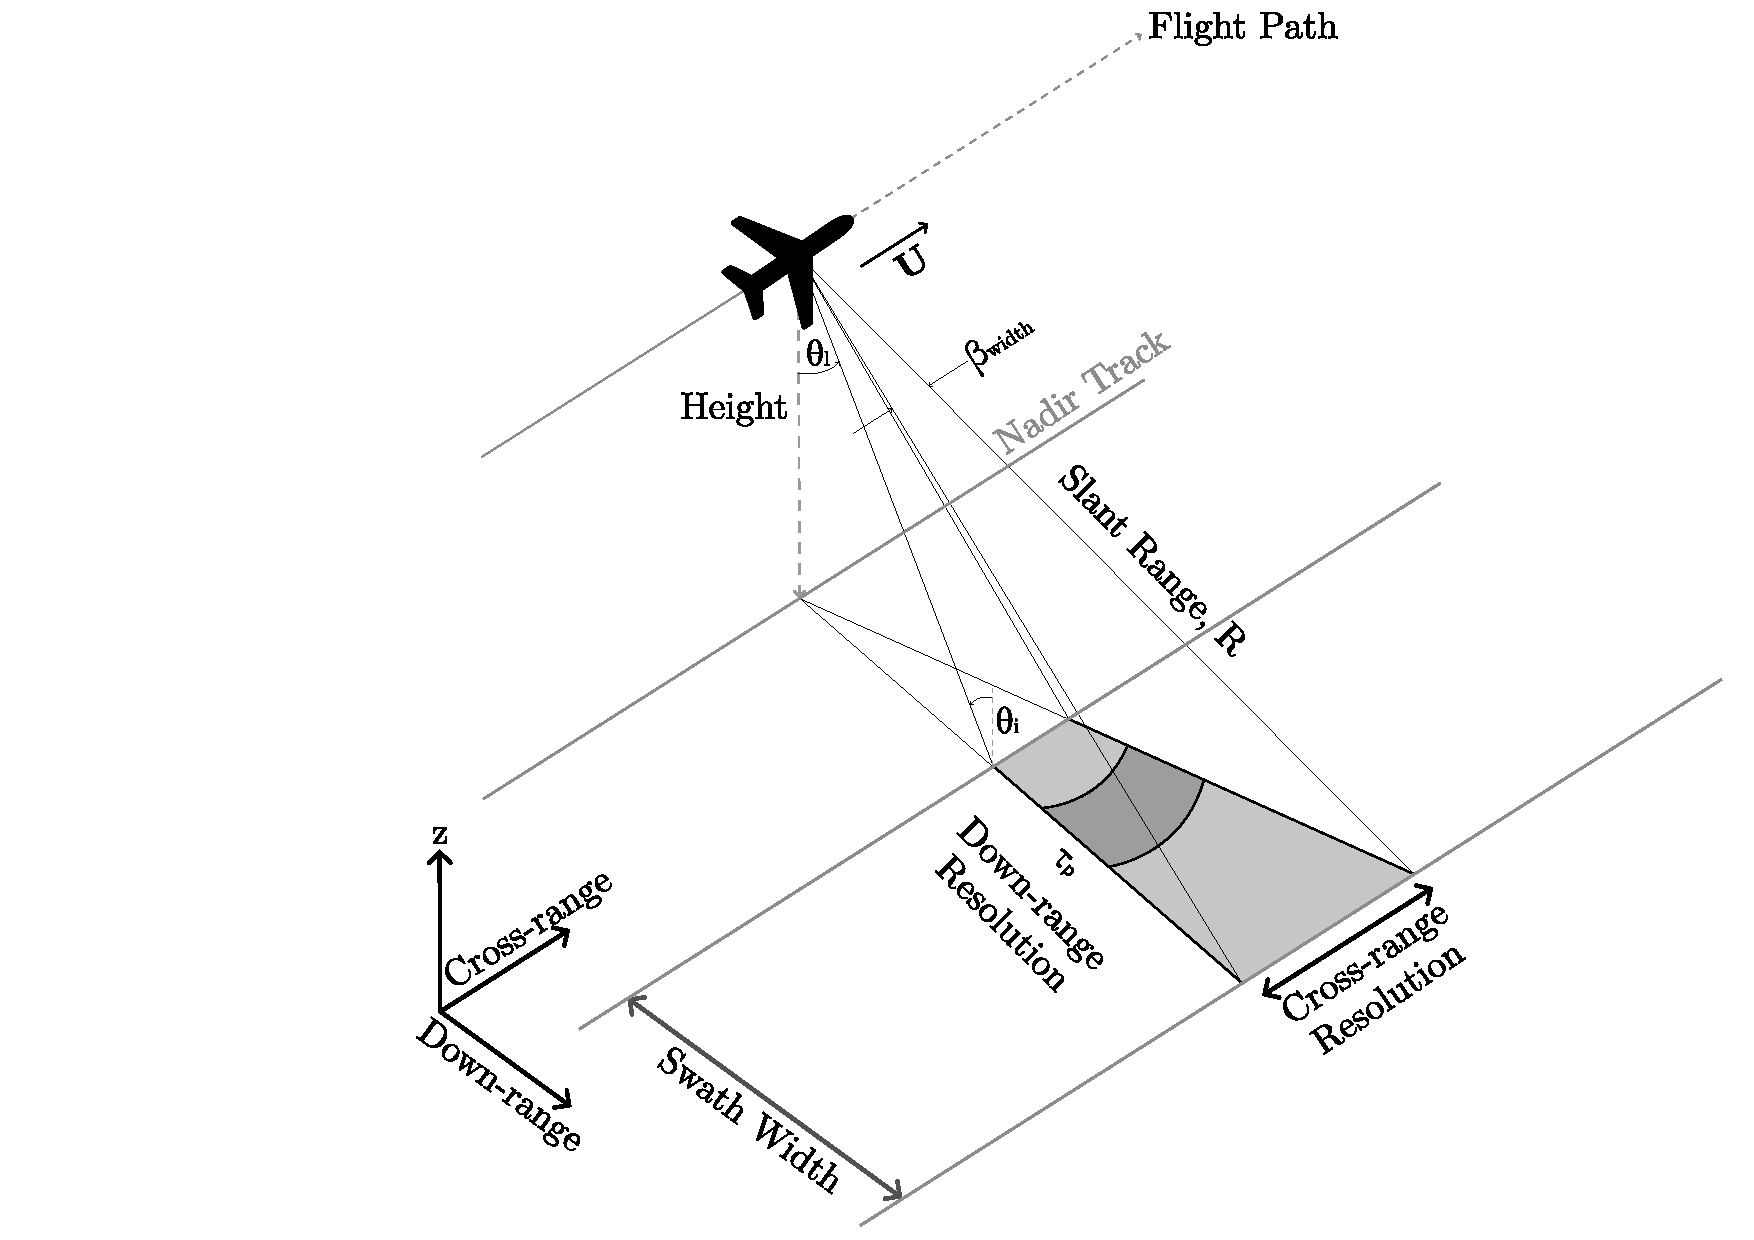
\includegraphics[width=.95\linewidth]{Figures/Theory/slarGeometry.pdf}
    \caption{Graphical representation of a \acs{slar} system with important features labelled. Adapted from \cite{Moreira2013,Meyer2019}.}
    \label{fig:theory.slarGeometry}
\end{figure}

The radar system operates by transmitting a series of chirps, each with a pulse length defined as $\tau_{p}$, which illuminate the region of the ground referred to as the antenna footprint \cite{Meyer2019}. To calculate the size of this footprint, consider the radar's slant range, $R$, which represents the distance between the antenna and its footprint, as well as the beamwidth, denoted as $\beta_{width}$. The beamwidth can be defined as the ratio between the radar's wavelength, $\lambda$, and the antenna length, $L_{ant}$. This definition enables the determination of the antenna footprint size, $S$ \cite{Meyer2019}

\begin{equation} \label{eq:rar.footprintSize}
    S \approx \frac{\lambda}{L_{ant}}R = \beta_{width} R \,\, \text{[m]}
\end{equation}

This footprint is shown in dark grey in Figure \ref{fig:theory.slarGeometry} as well as depicting the incidence angle, $\theta_{i}$, which can be derived as $90 \degree - \theta_{l}$. The resolution of this beamwidth in both the down-range and cross-range directions can be empirically determined. The slant range resolution of a \ac{slar} system is defined in terms of the speed of light, $c$ and the pulse length, $\tau_{p}$ as

\begin{equation} \label{eq:rar.slantRangeResolution}
    \delta_{sr} = \frac{c \tau_{p}}{2} \,\, \text{[m]}
\end{equation}

The resolution of a radar system allows it to differentiate between different objects at different slant ranges from the sensor \cite{Moreira2013}. It is also useful to define the down-range resolution in terms of the incidence angle and slant range resolution as

\begin{equation} \label{eq:rar.groundRangeResolution}
    \delta_{dr} = \frac{\delta_{sr}}{\text{sin}(\theta_{i})} \,\, \text{[m]}
\end{equation}

and the cross-range resolution as

\begin{equation} \label{eq:rar.crossrangeResolution}
  \delta_{cr} = \frac{\lambda}{L_{ant}}R \,\, \text{[m].}
\end{equation}

In order to see the drawback of \ac{rar} in terms of resolution, it is useful to apply values to Equation \ref{eq:rar.crossrangeResolution}. Consider an X-band\footnote{Give wavelength and freq of X-band} \ac{rar} radar system with a slant range to the target of 7\,km, as in a space-borne application, and with an antenna length of 5\,m. This yields a cross-range resolution of

\begin{gather*}
    \delta_{cr} = \frac{0.03\,\text{m}}{5\,\text{m}} \cdot 7000\,\text{m} = 42\,\text{m}
\end{gather*}

The above example shows that a space-borne application of \acs{rar} results in a loss of cross-range resolution. In the context of this project, this is impractical as ocean waves need to be imaged and differentiated between.

The limited resolution of \acs{rar} led to the development of \acs{sar}. This technology addresses the impact of antenna length by synthetically imitating a longer antenna length, which enhances the cross-range resolution. This is accomplished through exploiting the Doppler shift phenomenon and capturing multiple images of the same scene. For a more comprehensive understanding of the mathematical and signal processing aspects involved in generating a \acs{sar}, refer to \cite{Cumming2005}.


The synthetic length of the antenna \cite{Meyer2019} used in calculating the cross-range resolution can be determined as

\begin{equation} \label{eq:sar.virtualAntennaL}
    L_{SA} \approx \beta_{width}\cdot R 
\end{equation}

where the artificial beamwidth can be calculated as

\begin{equation} \label{eq:sar.beamwidth}
    \beta_{witdth_{SA}} = \frac{\lambda}{2L_{SA}}
\end{equation}

This, in turn, allows the cross-range resolution \cite{Moreira2013} for a \acs{sar} sensor to be calculated as

\begin{equation} \label{eq:sar.crossRangeResolution}
    \delta_{cr_{SA}} = R\cdot \beta_{SA} = R \cdot \frac{\lambda}{2L_{SA}} = \frac{L_{ant}}{2}
\end{equation}

Using the previous example of a space-borne sensor with an antenna of length, 5\,m, it can be seen that \acs{sar} improves the cross-range resolution when compared to \acs{rar}.

\begin{gather*}
    \delta_{cr_{SA}} = \frac{5\,\text{m}}{2} = 2.5\,\text{m}
\end{gather*}

This example shows that \acs{sar} allows fine cross-range resolution, a vital parameter in the application of imaging ocean waves. Along with this, \acs{sar} offers year-round imaging in any weather conditions as discussed in Section \ref{sec:litReview.sarCharac}.
% Check section ref

\subsection{\acs{sar} Imaging Modes} \label{subsec:theory.sar.imaging}
% SAR Imaging

Each \acs{sar} sensor can capture data in multiple modes with the most common modes being Spotlight, \ac{sm}, and ScanSAR. Sentinel-1A offers data products using three main capture modes: \acs{sm}, \ac{iw}, and \ac{ew} modes. \ac{iw} and \ac{ew} are both a new type of Scan\acs{sar} based on \ac{topsar}. These capture modes are shown visually in Figure \ref{fig:theory.sarCaptureModes} where $U$ represents the satellite's velocity.

%TOPS ref \cite{Huang2014}.


\begin{figure} [H]
    \centering
    \begin{subfigure}{0.48\textwidth}
        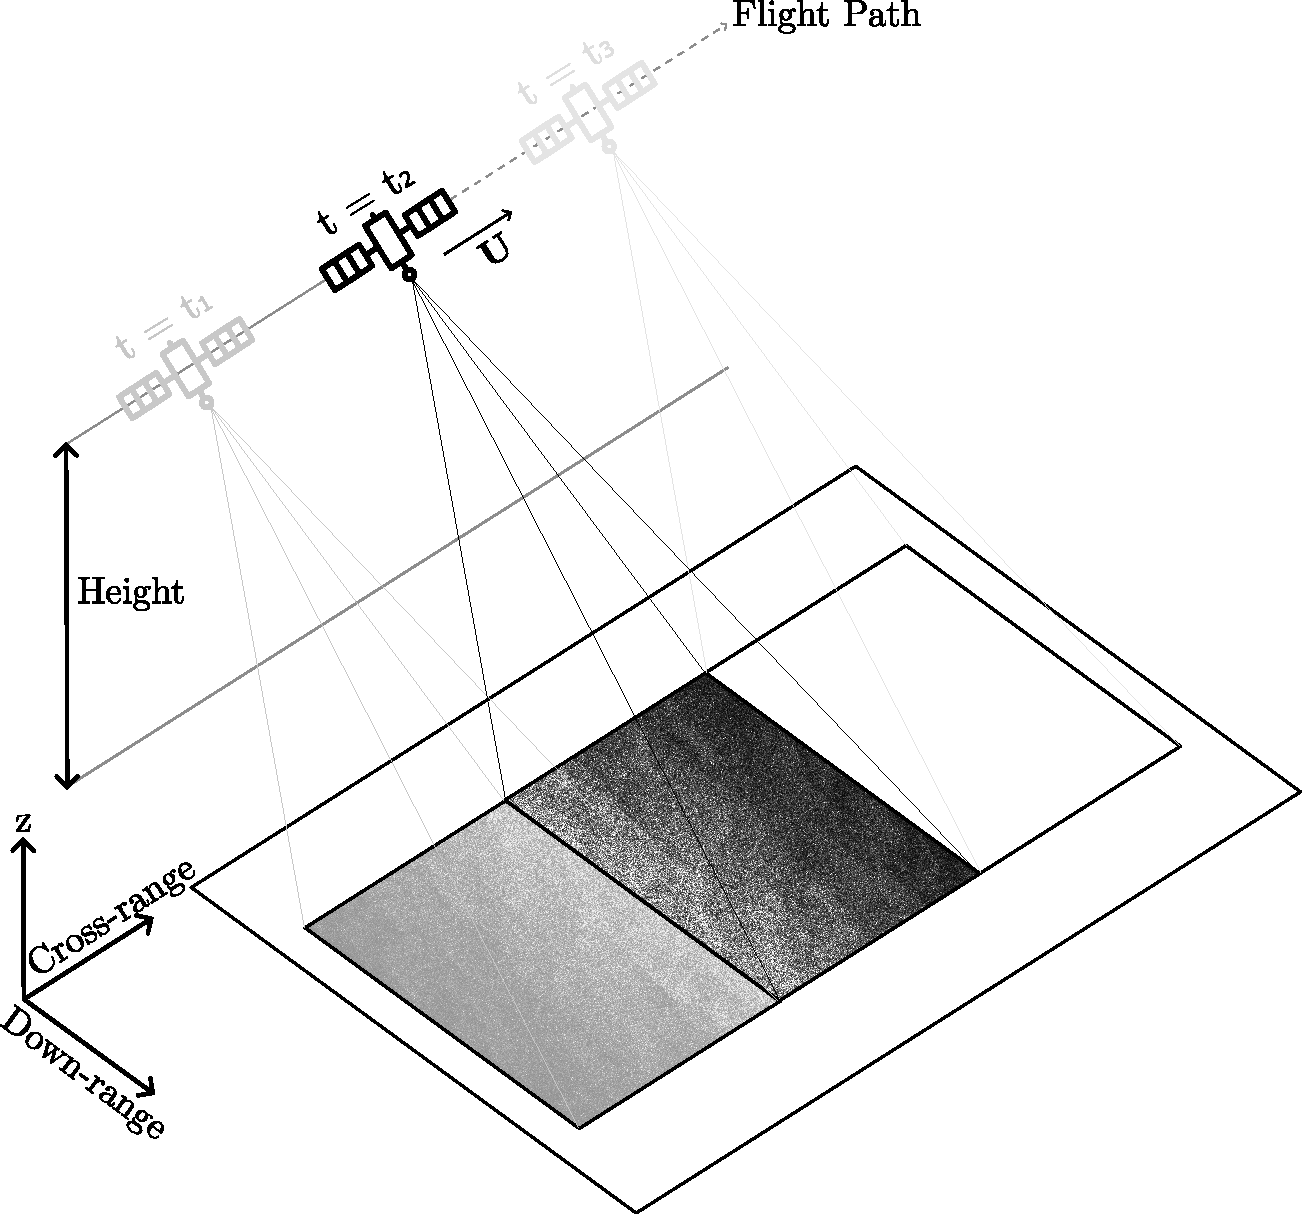
\includegraphics[width=\textwidth]{Figures/Theory/stripmap.pdf}
        \caption{\acf{sm} capture mode.}
        \label{fig:theory.stripmap}
    \end{subfigure}   
    \begin{subfigure}{0.48\textwidth}
        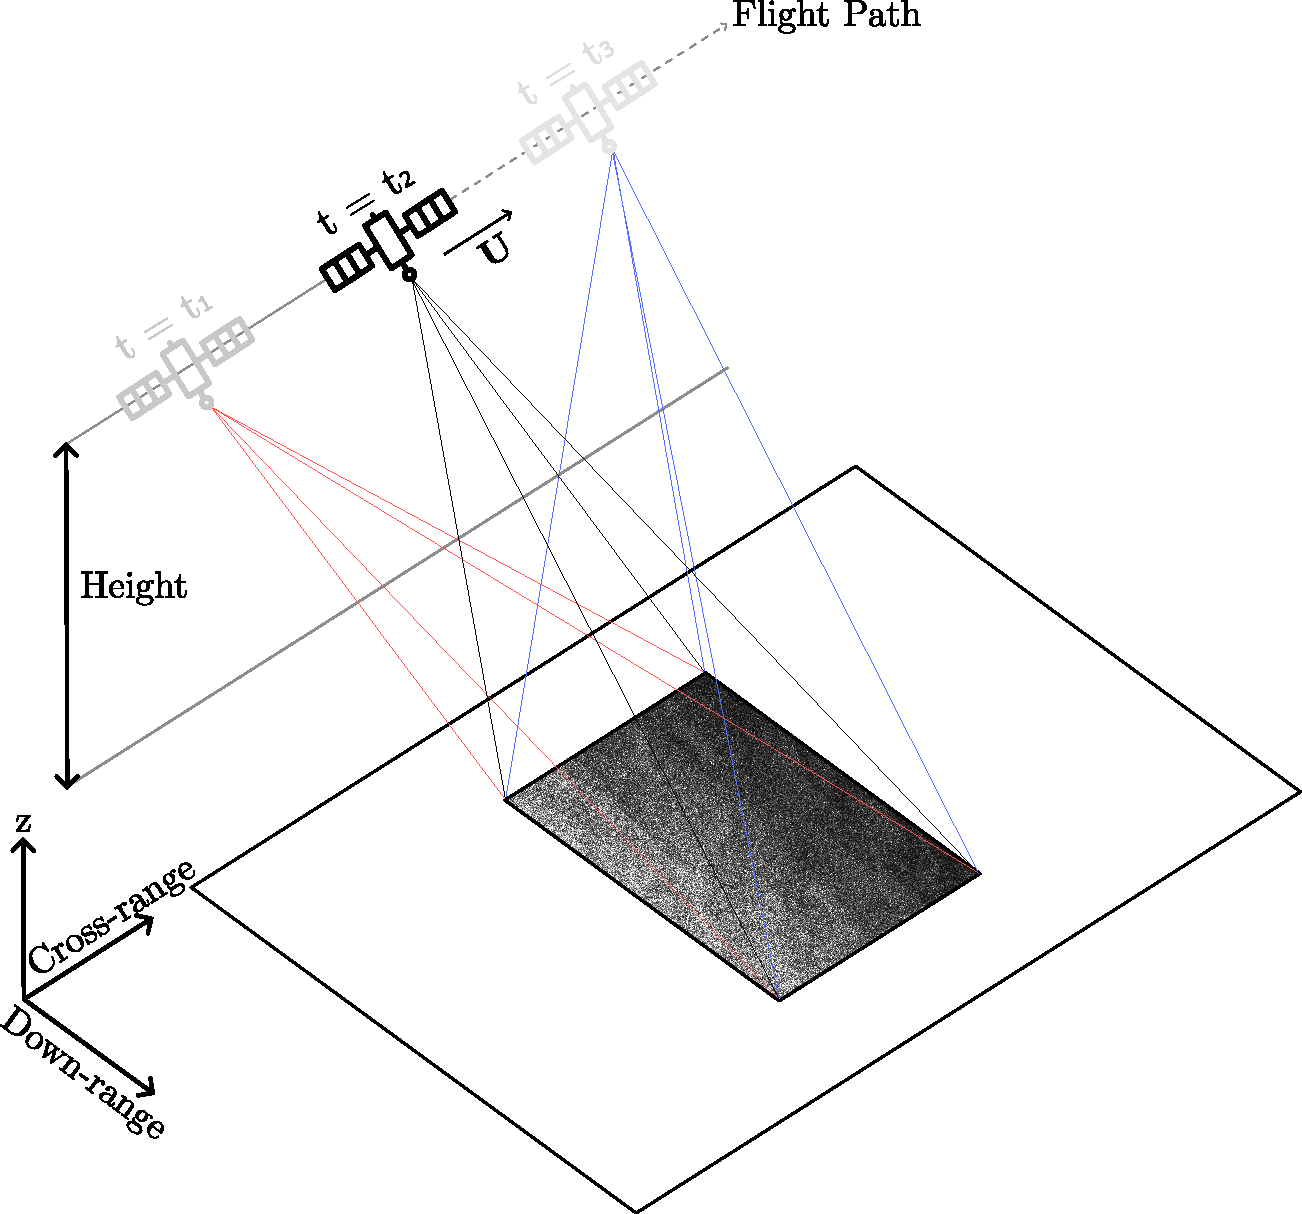
\includegraphics[width=\textwidth]{Figures/Theory/spotlight.pdf}
        \caption{Spotlight capture mode.}
        \label{fig:theory.spotlight}
    \end{subfigure} 
    \begin{subfigure}{0.48\textwidth}
        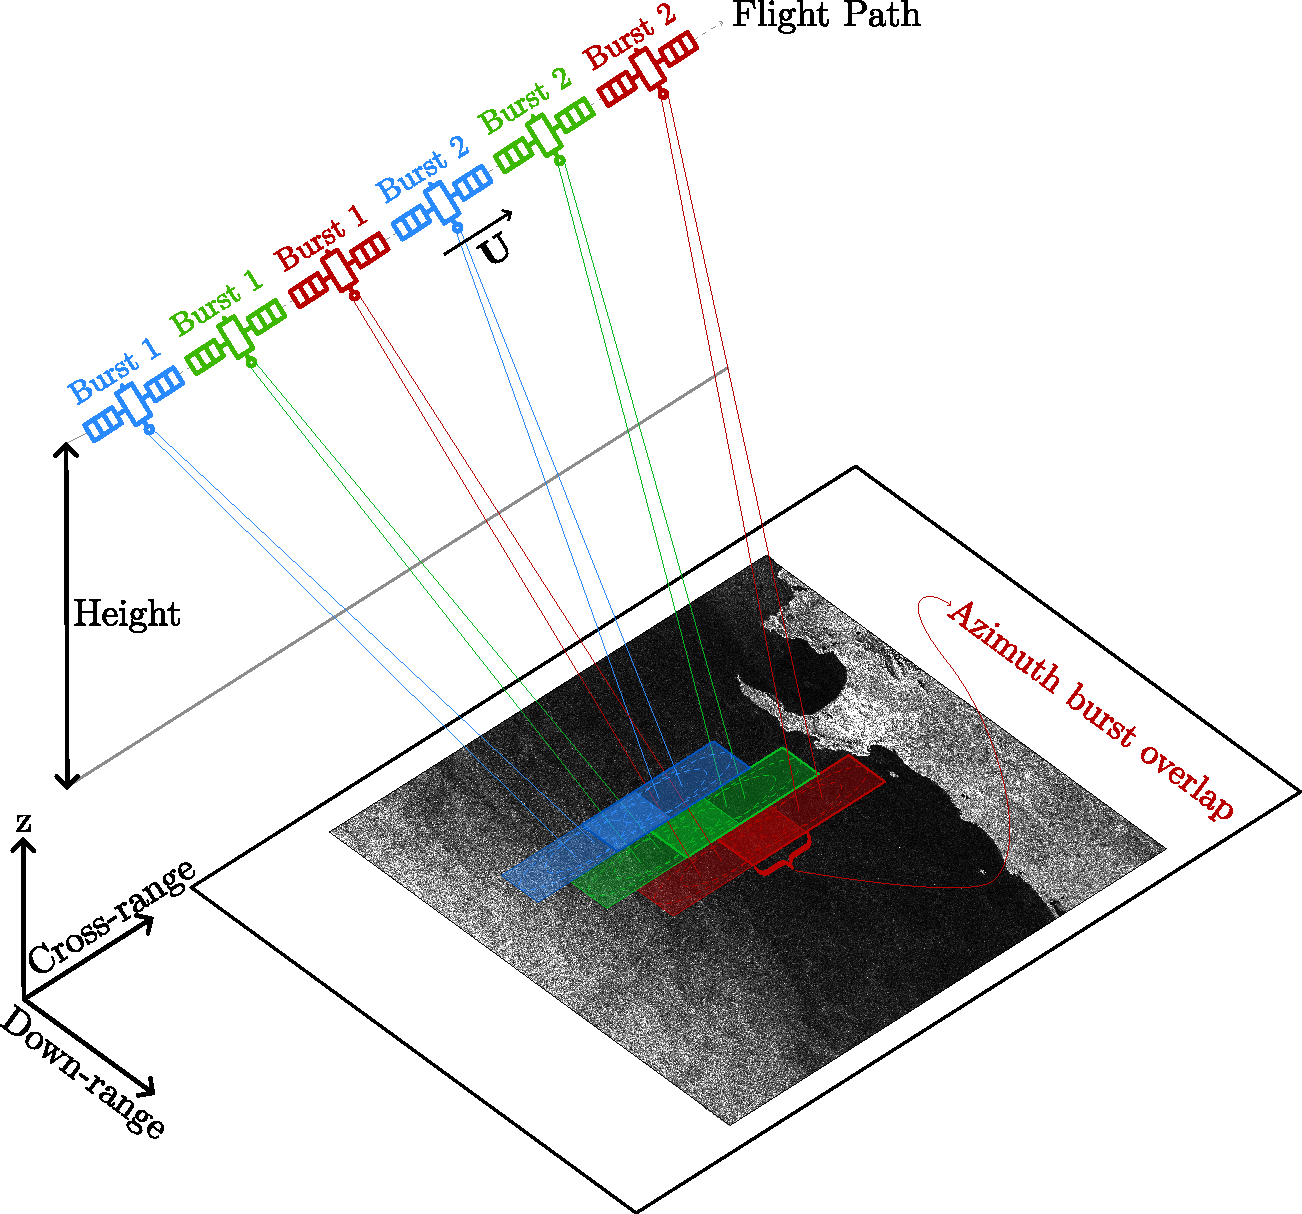
\includegraphics[width=\textwidth]{Figures/Theory/scanSAR.pdf}
        \caption{Scan\acs{sar} capture mode.}
        \label{fig:theory.scanSAR}
    \end{subfigure} 
    \begin{subfigure}{0.48\textwidth}
        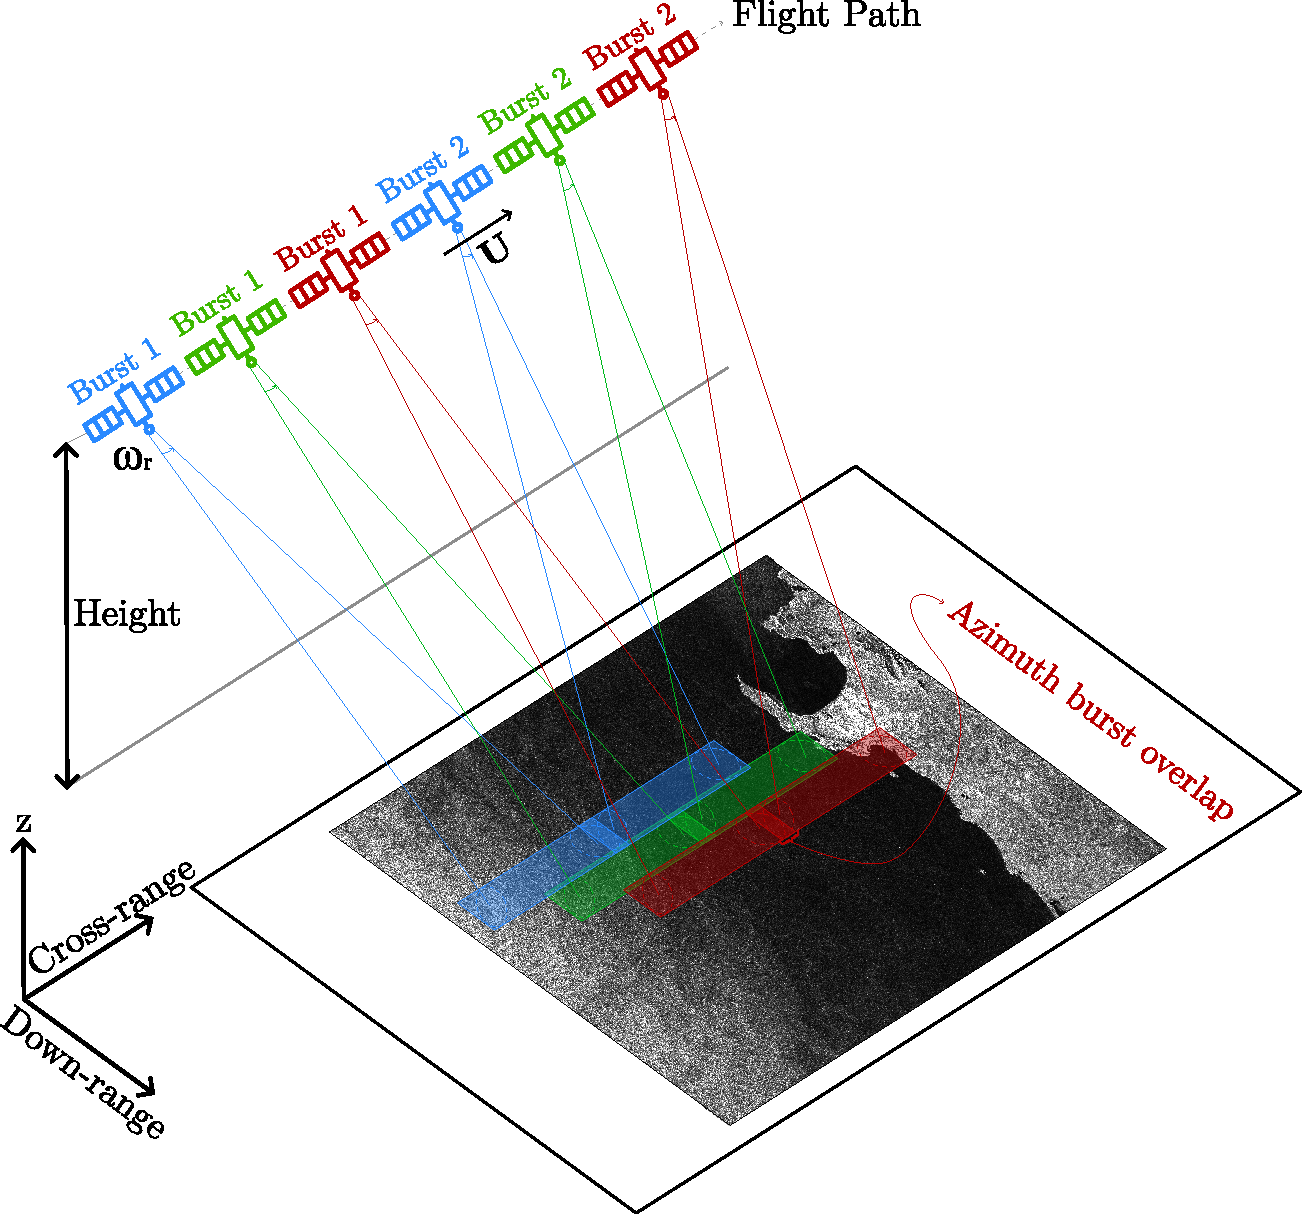
\includegraphics[width=\textwidth]{Figures/Theory/tops.pdf}
        \caption{\acs{topsar} capture mode used by \acs{s1a}. Adapted from \cite{Huang2014}.}
        \label{fig:theory.tops}
    \end{subfigure}     
    \caption{Graphical representation of commonly used \acs{sar} satellite capture and specific \acs{s1a} capture modes.}
    \label{fig:theory.sarCaptureModes}
\end{figure}

 % fix spelling and grammar of all

\subsubsection{\acf{sm} Mode}

\acs{sm} mode is the conventional \acs{sar} imaging mode \cite{Frery2022}. In \acs{sm} mode, the antenna has a fixed direction, which observes a fixed swath, whilst the satellite moves along its flight path \cite{Moreira2013} as depicted in Figure \ref{fig:theory.stripmap}. This allows a continuous ground swath to be illuminated with a continuous sequence of chirps. The echoes received back by the sensor are processed and combined to form a continuous image of the observed scene. \acs{sm} mode provides increased cross-range resolution as multiple echoes are received back from the same target within the scene. \acs{sm} mode is a versatile imaging mode as it allows detailed imagery over a large area to be obtained over a single, continuous strip at a constant incidence angle \cite{Moreira2013,Frery2022,sentinel1ProductDef}.


% \acs{sm} mode, is the conventional \acs{sar} imaging mode \cite{Frery2022}, and features a fixed antenna direction observing a constant swath while the satellite progresses along its flight path, as shown in Figure \ref{fig:theory.stripmap}. This mode enables continuous ground swath illumination via a sequence of chirps, leading to a continuous scene image. It offers enhanced cross-range resolution due to multiple echoes from the same target, making it versatile for detailed imaging over a large area at a consistent incidence angle \cite{Moreira2013, Frery2022, sentinel1ProductDef}.

\subsubsection{Spotlight Mode}

Spotlight mode is used for high-resolution \acs{sar} imaging \cite{Meyer2019}, and involves targeting a specific area while continuously illuminating and capturing echoes during satellite movement along its flight path, as depicted in Figure \ref{fig:theory.spotlight}. Antenna beam control can be achieved mechanically or electronically through beam steering \cite{Frery2022}. Spotlight mode improves both down- and cross-range resolutions. Whilst its spatial coverage is smaller compared to \acs{sm} mode. By extending the synthetic antenna's length, Spotlight mode enhances cross-range resolution, making it ideal for applications requiring maximum resolution whilst accepting reduced spatial coverage \cite{Moreira2013}.

% Spotlight mode is recommended for high-resolution \acs{sar} imaging \cite{Meyer2019}. In Spotlight mode, the radar antenna targets a specific area whilst continuously illuminating this area and capturing the received echoes whilst travelling along its flight path \cite{Frery2022,Moreira2013}, as depicted in Figure \ref{fig:theory.spotlight}. The antenna beam is controlled either mechanically, or electronically through beam steering \cite{Frery2022} to ensure that the desired target is continuously illuminated over the capture time as the satellite travels along its flight path. Spotlight mode enhances both the down- and cross-range resolutions. Whilst Spotlight mode has a smaller spatial coverage than \acs{sm} mode, it trades this off for increased resolution. Spotlight mode increases the cross-range resolution by increasing the length of the synthetic antenna and it is useful when maximum resolution is required for an application with decreased spatial coverage \cite{Moreira2013}.

\subsubsection{Scan\acs{sar} Mode}

Scan\acs{sar} mode provides improved spatial coverage compared to both \acs{sm} and Spotlight modes, although at the cost of reduced cross-range resolution \cite{Frery2022}. In Scan\acs{sar}, the antenna periodically sweeps over multiple sub-swaths associated with various antenna orientations \cite{Frery2022,Moreira2013}, as shown in Figure \ref{fig:theory.scanSAR}. Each sub-swath is illuminated by multiple chirps but for a shorter duration compared to \acs{sm} mode \cite{Moreira2013}. The loss in resolution is due to the fact that the synthetic antenna length is divided up across the sub-swaths \cite{Frery2022}.

% Scan\acs{sar} mode offers increased spatial coverage, through the increase in swath width, over both \acs{sm} and Spotlight mode at the cost of reduced cross-range resolution \cite{Frery2022}. Scan\acs{sar} mode operates by having the antenna periodically sweep over various sub-swaths associated with various antenna orientations \cite{Frery2022,Moreira2013}, as depicted in Figure \ref{fig:theory.scanSAR}. Each sub-swath is illuminated by multiple chirps, but for a shorter time than in \acs{sm} mode \cite{Moreira2013} and the antenna orientation is changed by varying the look angle, $\theta_{l}$ of the antenna. These sub-swaths are combined when processing the raw data and result in increased swath width, with decreased cross-range resolution when compared to \acs{sm} and Spotlight modes \cite{Moreira2013}. This loss in resolution is due to the fact that the synthetic antenna length is divided up across the sub-swaths \cite{Frery2022}.

\subsubsection{\acs{topsar} Mode}

\ac{topsar} is a specialised form of Scan\acs{sar} imaging used by \acs{s1a} in both \ac{iw} and \ac{ew} modes. It acquires data by transmitting bursts and periodically switching the antenna beam between adjacent sub-swaths, as illustrated in Figure \ref{fig:theory.tops}. While Scan\acs{sar} uses mechanical or electronic beam steering, \acs{topsar} exclusively uses electronic beam steering in both down- and cross-range directions. \acs{topsar} offers the same spatial coverage as Scan\acs{sar} but with marginally improved cross-range resolution due to shorter burst times \cite{DeZan2006}. Consequently, \acs{topsar} is ideal for applications demanding high resolution and extensive swath coverage.

\acs{s1a}'s \acs{iw} mode uses \acs{topsar} imaging, retaining wide swath coverage and improved cross-range resolution \cite{sentinel1ProductDef}. \acs{iw} mode consists of three wide sub-swaths captured by steering the antenna in the cross-range direction by an angle $\omega_{r}$ \cite{sentinel1ProductDef}. On the other hand, \acs{ew} mode, also based on \acs{topsar} imaging, differs in the number of sub-swaths used for complete scene capture. While \acs{iw} mode utilises three sub-swaths, \acs{ew} mode employs five wide sub-swaths to construct the entire image, effectively enhancing spatial coverage while maintaining cross-range resolution.

% \ac{topsar} is a specialised form of Scan\acs{sar} imaging used by \acs{s1a} in both \ac{iw} and \ac{ew} modes. \acs{topsar} captures data by transmitting bursts whilst periodically switching the antenna beam between adjacent sub-swaths \cite{DeZan2006}, as depicted in Figure \ref{fig:theory.tops}. Whilst Scan\acs{sar} uses mechanical or electronic beam steering, \acs{topsar} utilises only electronic beam steering and does this in both the down- and cross-range directions. \acs{topsar} offers the same spatial coverage as Scan\acs{sar}, whilst marginally improving cross-range resolution due to shorter burst times when compared to Scan\acs{sar} \cite{DeZan2006}. Thus, \acs{topsar} is useful for high-resolution and large swath applications. 

% \acs{iw} mode implemented by \acs{s1a} utilises \acs{topsar} imaging and maintains the wide swath coverage and improved cross-range resolution \cite{sentinel1ProductDef}. \acs{iw} captures are made up of three wide sub-swaths \cite{sentinel1ProductDef} captured by beam steering the antenna in the cross-range direction through an angle, $\omega_{r}$. \ac{ew} mode is also based on \acs{topsar} imaging techniques and differs from \acs{iw} mode in the number of sub-swaths which are used when capturing the full scene. Where \acs{iw} mode uses three sub-swaths, \acs{ew} mode utilises five wide sub-swaths to construct the full image whilst maintaining cross-range resolution and increasing the spatial coverage of the capture.

Table \ref{tab:theory.s1aImagingParams} provides a comparison of the ground resolution of all \acs{s1a} imaging techniques for \acs{grd} data.

\begin{table}[H]
\centering
\begin{tabular}{|c|c|c|}
\hline
\textbf{Mode} & \multicolumn{1}{l|}{\textbf{Minimum Ground Swath Width {[}km{]}}} & \multicolumn{1}{l|}{\textbf{Resolution (dr x cr) {[}m{]}}} \\ \hline
\textbf{\acs{sm}} & 80 & 10x10 \\ \hline
\textbf{\acs{iw}} & 250 & 10x10 \\ \hline
\textbf{\acs{ew}} & 410 & 25x25 \\ \hline
\end{tabular}
\caption{Comparison of ground swath width and resolution of \acs{s1a} imaging modes. Adapted from \cite{sentinel1ProductDef}}
\label{tab:theory.s1aImagingParams}
\end{table}

Due to the fact that this project requires imaging ocean waves, fine-range resolution is required. To this end, data products captured using \acs{sm} or \acs{iw} mode are utilised due to their improved resolution over \acs{ew} mode depicted in Table \ref{tab:theory.s1aImagingParams}.




% \subsubsection{Data Levels}

% \begin{itemize}
%     \item Data levels (Level 0 - I and Q, Level 1 - GND)
% \end{itemize}

\subsection{Pre-processing Techniques} \label{subsec:theory.sar.preProcess}

\textbf{Speckle}

Speckle, often noted for its "salt-and-pepper" appearance \cite{Meyer2019} in \acs{sar} images, results from the interference of multiple scatters within a resolution cell which leads to varying intensity values. Even when imaging a uniform surface, speckle exists due to phase variations amongst scatterers within the resolution cell, with brighter image regions exhibiting more intense speckle \cite{Moreira2013,Meyer2019}. Speckle is not an error in a \acs{sar} image, but a consequence of imaging with finite resolution. Higher resolution weakens the speckle effect as it reduces the number of scatterers within the resolution cell \cite{Meyer2019}. Unprocessed intensity VV \acs{grd} data is shown in Figure \ref{fig:theory.data.unprocessed} and speckle can be seen in both sub-scenes.

\begin{figure}[H]
    \centering
    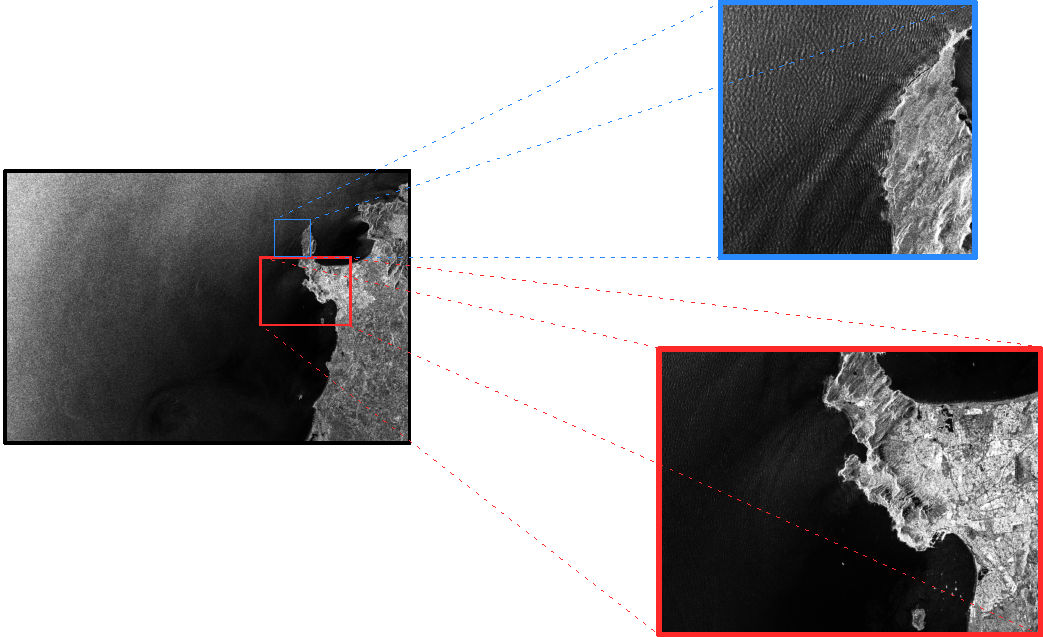
\includegraphics[width=0.85\textwidth]{Figures/Theory/unprocessedSARData.pdf}
    \caption{Unprocessed \acs{grd} \acs{s1a} data.}
    \label{fig:theory.data.unprocessed}
\end{figure}

\textbf{Thermal Noise}
% Check spelling and grammar

Thermal noise significantly affects \acs{sar} image quality. It represents inherent background energy generated by the radar receiver channel and creates a noise threshold. When a received signal falls below this threshold, it becomes indistinguishable from thermal noise, which impacts low-intensity scatterers, such as new ice and open water \cite{Carsey1992}, especially in cross-polarised applications. In these cases, the thermal noise can significantly impact the interpretability of the \acs{sar} data \cite{Carsey1992}. Unlike speckle, which appears as grainy patterns and can be reduced through filtering, thermal noise is characterised by a uniform background noise level. In the context of \acs{s1a}, thermal noise is composed of two additive noise sources related to antenna movement and scalloping noise\footnote{Define scalloping noise}. It predominantly affects \acs{topsar} imaging mode, especially for cross-polarised images.

% Thermal noise is a significant factor in \acs{sar} imaging as it influences the quality of these images. Thermal noise represents the inherent background energy generated by the radar receiver channel \cite{Park2018}. Thermal noise is responsible for creating a noise threshold for a \acs{sar} image. When a received signal drops below this noise threshold, it becomes nearly indistinguishable from the thermal noise. This poses an issue for analysing scatterers which return low-intensity values, such as new ice and open water \cite{Carsey1992}. In these cases, the thermal noise can significantly impact the interpretability of the \acs{sar} data \cite{Carsey1992}.

% While speckle noise appears as grainy patterns across the image and can often be reduced by filtering techniques \cite{Meyer2019}, thermal noise is characterized by a uniform, background noise level. Speckle noise is a result of the coherent nature of \acs{sar} imaging, leading to constructive and destructive interference of radar signals. Thermal noise, on the other hand, results from the receiver's inherent noise and significantly impacts low backscatter targets, especially in cross-polarised channels \cite{Park2018,Park2019}.

% In the context of \acs{s1a}, thermal noise plays an important role. Thermal noise is comprised of two sources of additive noise. The first is linked to the movement of the antenna and causes variability in the down-range direction. The second is known as scalloping noise\footnote{define scalloping noise} and varies in the cross-range direction \cite{Park2019}. Thermal noise impacts \acs{topsar} imaging mode more than others, particularly for cross-polarised images \cite{Park2018}. Furthermore, \acs{s1a} \acs{ew} mode \acs{sar} images, particularly those acquired over regions with a low backscatter, such as calm oceans and young smooth sea ice, are susceptible to thermal noise \cite{Carsey1992}.

Removal of \acs{s1a} thermal noise results in improved image quality and can be visually seen in Figure \ref{fig:theory.data.thermalNoiseRemoval} when compared to Figure \ref{fig:theory.data.unprocessed}, particularly over land regions in the second sub-scene.

\begin{figure}[H]
    \centering
    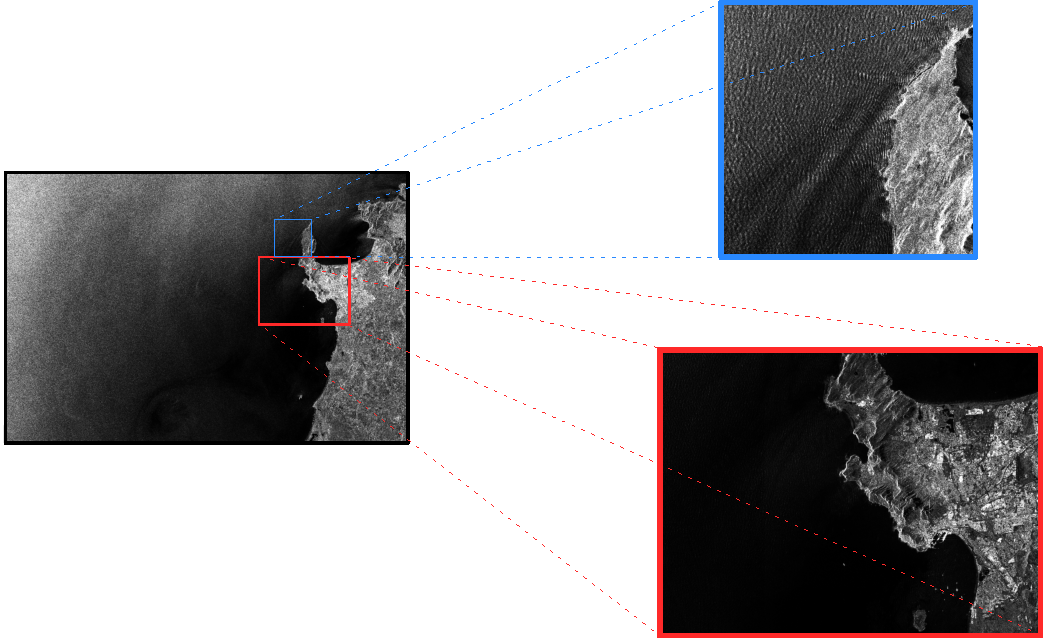
\includegraphics[width=0.85\textwidth]{Figures/Theory/thermalNoiseCalibratedSARData.pdf}
    \caption{\acs{grd} \acs{s1a} data with thermal noise removed using \acs{snap}.}
    \label{fig:theory.data.thermalNoiseRemoval}
\end{figure}

\subsubsection{Radiometric Calibration}
% Reword

In \acs{sar} imaging, $\sigma_{0}$ represents the backscatter coefficient, which indicates the radar signal's strength reflected by scatterers. $\sigma_{0}$ is a dimensionless number that accounts for variations in factors like incidence angle, wavelength, polarisation, and surface properties. Radiometric calibration addresses \ac{rcs} variations, ensuring that pixel values in \acs{sar} images are both qualitatively representative and quantitatively aligned with $\sigma_{0}$. This process corrects radiometric bias present in raw \acs{sar} data, enabling its use in quantitative applications like target recognition and environmental monitoring. Calibration factors in the scattering area, antenna gain pattern, and range spread loss, enhance the accuracy and reliability of \acs{sar} data.

% Fact check
Radiometric calibration of \acs{s1a} \acs{grd} data can be visually seen in Figure \ref{fig:theory.data.radiometric} over mountainous regions in both sub-scenes. This is due to the correction of backscatter bias which doesn't account for elevation changes.

% In \acs{sar} imaging, $\sigma_{0}$ is known as the backscatter coefficient and acts as an indicator of the strength of radar signals reflected by scatterers. It provides a normalised dimensionless number that allows for comparing the observed signal strength to what would be expected from a standard one-square-meter area \cite{ElDarymli2014}. It's important to emphasise that $\sigma_{0}$ exhibits significant variations based on factors such as incidence angle, wavelength, polarisation, and the properties of the scattering surface itself. 

% Radiometric calibration in SAR images is a vital process, and it primarily involves addressing the variations in \acs{rcs}, which quantifies the radar signal's strength reflected by distributed scatterers. Calibration ensures that pixel values in \acs{sar} images are not only qualitatively representative but also quantitatively aligned with the \acs{rcs} and backscatter coefficient, $\sigma_{0}$. Essentially, radiometric calibration rectifies the radiometric bias present in the raw \acs{sar} data, making it suitable for a wide array of quantitative applications. This calibration process includes adjustments for factors like scattering area, antenna gain pattern, and range spread loss, guaranteeing the accuracy and reliability of \acs{sar} data for applications such as target recognition and environmental monitoring.

% Update calibrated image
\begin{figure}[H]
    \centering
    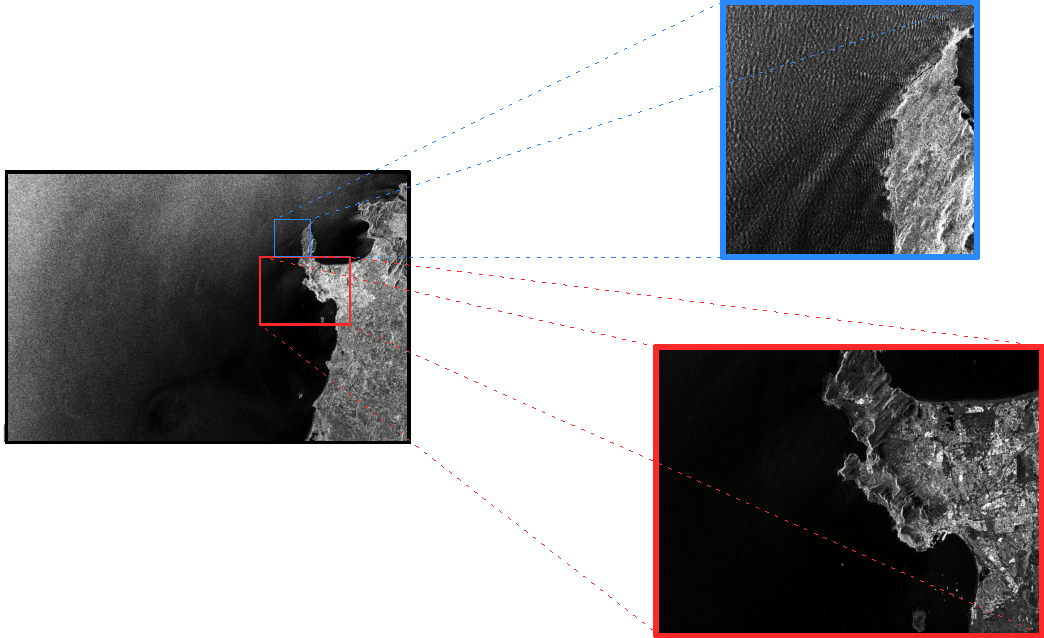
\includegraphics[width=0.85\textwidth]{Figures/Theory/radiometricCalibratedSARData.pdf}
    \caption{Radiometrically calibrated \acs{grd} \acs{s1a} data done using \acs{snap}.}
    \label{fig:theory.data.radiometric}
\end{figure}

\begin{itemize}
    \item Mention geocoding and terrain rectification (Link why this is the case)
    \item Speak about speckle (or link)
    \item Thermal Noise Removal
    \item Radiometric calibration
    \item Show graphically what each technique does and how it changes the image (Maybe in the appendix)
\end{itemize}

\subsection{Polarisation} \label{subsec:theory.sar.polarisation}

Polarisation is a fundamental aspect of \acs{sar} imaging. Polarisation refers to the orientation of the plane in which an \acs{em} wave oscillates as it propagates. Linear polarisation maintains a constant orientation along the wave's path, while circular and elliptical polarisations involve changing oscillation plane orientations, forming shapes like ellipses or circles \cite{Meyer2019}.

Traditionally, most \acs{sar} systems used single-polarised sensors, predominantly operating in HH (horizontal transmit, horizontal receive) or VV (vertical transmit, vertical receive) polarisation. However, newer \acs{sar} sensors offer dual-polarisation or quad-polarisation capabilities. These sensors can transmit both horizontally and vertically polarised waveforms and receive signals from both polarisations. Understanding the polarisation of a \acs{sar} image is crucial as it affects how radar signals interact with objects on the ground, influencing the recorded radar brightness for specific polarisations.

To interpret polarimetric SAR data effectively, it is helpful to consider how different types of scatterers interact with different polarizations. Rough surface scatterers, double-bounce scatterers, and volume scatterers make up the three primary categories of scatterers in a scene. Different polarimetric channels exhibit varying preferences for these scattering types, and these preferences can be used to analyse and classify scattering types. 


\subsubsection{Scattering}

Scattering is important to understand how satellite sensors detect and interpret \acs{em} waves. Scattering on the Earth's surface involves two primary processes: surface and volume scattering. Surface roughness plays a critical role in \acs{em} backscatter. A flat or specular surface\footnote{Define specular surface} behaves like a mirror, reflecting radiation back to the sensor only when the surface aligns perpendicularly with the sensor's line of sight. This occurs with flat or tilted surfaces, such as mountains or ocean surface waves. In contrast, rougher surfaces scatter a portion of incident EM radiation back toward the sensor. 

When the surface has a regular structure, such as waves with a specific wavelength, it can result in positive interference, a phenomenon known as Bragg scattering. Bragg scattering is of particular interest in the context of ocean waves and is caused by short ripple waves on the ocean surface \cite{Hasselmann1991}. This phenomenon is characterised by the constructive interference of incoming and backscattered \acs{em} radiation due to the regular structure of waves. This creates high backscatter values. The key factor for Bragg scattering's occurrence is the consistency between the wavelength of the electromagnetic waves and the spacing between wave crests.

% Bragg scattering enables radar instruments like scatterometers and Synthetic Aperture Radar (SAR) sensors to capture information about surface waves on the ocean, aiding in various applications like wave height and wind speed retrieval. 

%This effect is especially prominent at microwave frequencies, where ripple waves on water have wavelengths on the order of the EM wavelength. 



\begin{figure} [H]
    \centering
    \begin{subfigure}{0.31\textwidth}
        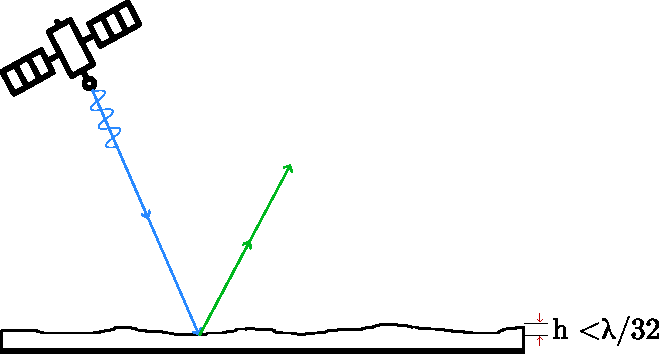
\includegraphics[width=\textwidth]{Figures/Theory/smoothSurface.pdf}
        \caption{\textbf{Smooth surface} \\ Near-perfect specular reflection.}
        \label{fig:theory.data.surface.smooth}
    \end{subfigure}   
    \begin{subfigure}{0.35\textwidth}
        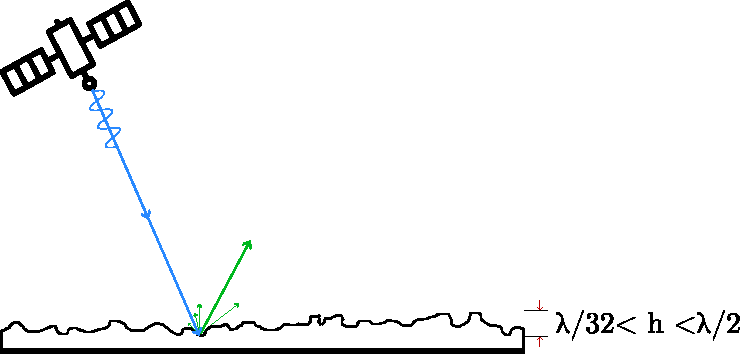
\includegraphics[width=\textwidth]{Figures/Theory/intermediateSurface.pdf}
        \caption{\textbf{Intermediate surface} \\ Moderate signal return.}
        \label{fig:theory.data.surface.intermediate}
    \end{subfigure} 
    \begin{subfigure}{0.31\textwidth}
        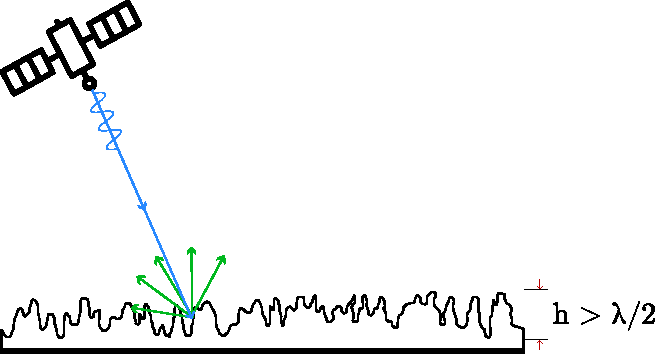
\includegraphics[width=\textwidth]{Figures/Theory/roughSurface.pdf}
        \caption{\textbf{Rough surface} \\ Diffuse scattering.}
        \label{fig:theory.data.suface.diffuse}
    \end{subfigure}    
    \caption{Comparison of surface roughness and surface backscatter. Adapted from \cite{Meyer2019}.}
    \label{fig:theory.data.surface}
\end{figure}

% Scatterers, surface roughness and penetration of wavelength (NEEED NEW TITLE)
% Speckle - Page 918 of PoMR
%   - Page 148 of Radar Imaging of Ocean Waves
\begin{itemize}
    \item Penetration of radar signals (Link to wavelength)
    \item - In the context of this work (Ocean waves [bragg scattering of wind-generated ripple waves] and sea ice)
    \item Surface roughness
    \item Scattering types
\end{itemize}

\begin{itemize}
    \item Speak about different polarisations and why each is good at what it does (In wave, ocean and land context)
    \item Visually show how each differs
    \item Focus on VV and HH and why they are used for Hasselmann in the context of ocean waves
\end{itemize}

%====================================================
% SAR OCEAN WAVE INVERSION
%====================================================
% \section{\acs{sar} Ocean Wave Inversion} \label{sec:theory.oceanWaveInversion}
% % Explain link to sea ice and wave modelling
% \subsection{Hasselmann and Hasselmann Inversion Technique} \label{subsec:theory.oceanWaveInversion.Hasselmann}
\section{Hasselmann and Hasselmann Ocean Wave Inversion Technique} \label{sec:theory.hasselmann}
The \ac{hh} process maps an ocean wave spectrum, as described in Section \ref{sec:theory.waves}, into a \ac{sar} image spectrum, as described in Section \ref{sec:theory.sar}. The \ac{hh} inversion procedure consists of two main parts - the \acs{sar} imaging of ocean waves, followed by an inversion to extract a wave spectrum. A full derivation of the \ac{hh} procedure is given in Appendix \ref{ap:hh}, however, an overview of the procedure, along with the relevant formulas is given in the following section.

%\subsubsection{\acs{sar} Imaging of Ocean Waves} \label{subsubsec:theory.oceanWaveInversion.Hasselmann.sarImaging}
\subsection{\acs{sar} Imaging of Ocean Waves} \label{subsec:theory.hasselmann.sarImaging}

\acs{hh} \cite{Hasselmann1991} state that the waves captured by a \acs{sar} spectrum are modulated through three different modulation processes. Firstly, the change in incidence angle is due to the change in the slope of the wave face. Secondly, the interactions between short and long waves, which modulate the energy and wave number of the short, Bragg scattering, ripple waves. And thirdly, the orbital velocity of the long waves, which produces a Doppler shift in the received, return signal. This causes an azimuthal displacement of the scatterers in the \acs{sar} image. This third modulation process is known as velocity bunching and is the main cause of nonlinearity in the imaging of ocean waves. All three of these modulation processes can be represented by their respective modulation transfer functions, and are denoted by the general form, $T^x_k$.

In order to derive a \acs{sar} spectrum from an ocean wave spectrum, \acs{hh} treat the captured \acs{sar} image as two separate procedures, namely the frozen surface, defined by the \ac{rar} imaging mechanism, and the motion effects, related to \acs{sar} imaging. The reason these motion effects arise is due to the way in which a \acs{sar} image is captured, as discussed in Section \ref{subsec:theory.sar.imaging}.

\subsubsection{Frozen Surface Contribution} \label{subsubsec:theory.hasselmann.sarImaging.frozenSurface}

%\textit{\textbf{Frozen Surface Contribution}}

The \ac{rar} \ac{mtf} \cite{Hasselmann1991} can be defined as 

\begin{equation} \label{eq:hh.rar.TR_k_sum}
    T^R_k = T^t_k + T^h_k
\end{equation}

where $T^t_k$ and $T^h_k$ are the tilt and hydrodynamic interaction \acp{mtf} respectively \cite{Hasselmann1991}. These two \acp{mtf} are defined as follows.

\begin{subequations}  \label{eq:hh.rar.Tt_k}
  \begin{align}
    \text{For VV Polarisation: } T^t_k = 4ik_{l}\text{cot}\left ( \theta_{i}  \right )\left (1+\text{sin}^2\theta_{i}  \right )^{-1} \\
    \text{For HH Polarisation: } T^t_k = 8ik_{l}\left (\text{sin}2\theta_{i}  \right )^{-1}
  \end{align}
\end{subequations} 

Where $\theta_{i}$ represents the radar incidence angle and $k_{l}$ represents the component of the wave-number vector in the radar look direction. These coordinates are chosen such that the $x$-axis represents the \acs{sar} satellite flight direction, and the $y$-axis points in the positive or negative look direction, $l$, for a left or right looking \acs{sar} satellite respectively \cite{Hasselmann1991}. 

\begin{equation} \label{eq:hh.rar.Th_k}
    T^h_k = \frac{\omega - i\mu}{\omega^2 + \mu^2}(4.5)k\omega \left ( \frac{k_y^2}{k^2}  \right )
\end{equation}

Where $k$ is the wave number vector and $\omega = \sqrt{gk}$.

\subsubsection{Motion Effects} \label{subsubsec:theory.hasselmann.sarImaging.motionEffects}
%\subparagraph{Motion Effects:}

The range velocity \acs{mtf} \cite{Hasselmann1991} can be defined as

\begin{equation} \label{eq:hh.motion.Tv_k}
    T^v_k = -\omega \left ( \text{sin}(\theta_{i})\frac{k_l}{\left | k \right |} +icos(\theta_{i}) \right )
\end{equation}

and the velocity bunching \acs{mtf} \cite{Hasselmann1991} can be defined as

\begin{equation} \label{eq:hh.motion.Tvb_k}
    T^{vb}_k = -i\beta k_{x} T^v_k
\end{equation}

where $\beta$ is the ratio of slant range, $R$, and satellite velocity, $U$; $\beta = R/U$ \cite{Hasselmann1991}. Defining the velocity bunching \acs{mtf} allows the net \acs{sar} imaging \acs{mtf} \cite{Hasselmann1991}be defined as

\begin{equation} \label{eq:hh.motion.TS_k}
    T^{S}_k = T^R_k +  T^{vb}_k
\end{equation}

\subsubsection{Co/Autocovariance Functions} \label{subsubsec:theory.hasselmann.sarImaging.autocovarFunc}

The \acp{mtf} described in Equations \ref{eq:hh.rar.TR_k_sum}, \ref{eq:hh.rar.Tt_k}, \ref{eq:hh.rar.Th_k}, \ref{eq:hh.motion.Tv_k} allow three covariance functions to be defined. These are the orbital velocity covariance function, $f^v(\underline{r})$, the autocovariance function of \ac{rar} image intensity, $f^R(\underline{r})$, and the covariance function of \ac{rar} image intensity and nonlinear velocity, $f^{Rv}(\underline{r})$ \cite{Hasselmann1991}.

\begin{equation} \label{eq:hh.var.fv}
    f^v(\underline{r}) = \int E(\underline{k}) \left | T^v_k \right |^2 e^{i\underline{k}\cdot \underline{r}} d\underline{k}
\end{equation}

\begin{equation} \label{eq:hh.var.fR}
    f^R(\underline{r}) = \frac{1}{2}\int\left [ E(\underline{k}) \left | T^R_k \right |^2  + E(-\underline{k}) \left | T^R_{-k} \right |^2\right ] e^{i\underline{k}\cdot \underline{r}} d\underline{k}
\end{equation}

\begin{equation} \label{eq:hh.var.fRv}
    f^{Rv}(\underline{r}) = \frac{1}{2}\int\left [ E(\underline{k}) T^R_k (T^v_k)^* + E(-\underline{k}) T^R_{-k} (T^v_{-k})^*\right ] e^{i\underline{k}\cdot \underline{r}} d\underline{k}
\end{equation}

\subsubsection{Spectral Expansion} \label{subsubsec:theory.hasselmann.sarImaging.spectralExpansion}
%\textbf{Spectral Expansion}

The functions described in Equations \ref{eq:hh.var.fv}, \ref{eq:hh.var.fR} and \ref{eq:hh.var.fRv} can, using the Fourier Transform, be expanded into spectral expansion terms using the following equations. $\Omega_n$ is the Fourier Transform operator given by $\frac{1}{4\pi}\int d\underline{r}e^{-i\underline{k}\cdot \underline{r}}$ \cite{Hasselmann1991}, which represents a two-dimensional \ac{fft}.

\begin{equation} \label{eq:hh.ft.2n}
    P^S_{n,2n} = \Omega_n \left \{ \frac{f^v(\underline{r})^n}{n!} \right \}
\end{equation}

\begin{equation} \label{eq:hh.ft.2n-1}
    P^S_{n,2n-1} = \Omega_n \left \{ \frac{i\left [ f^{Rv}(\underline{r}) - f^{Rv}(-\underline{r}) \right ] f^v(\underline{r})^{n-1}}{(n-1)!} \right \}
\end{equation}

\begin{equation} \label{eq:hh.ft.2n-2}
    P^S_{n,2n-2} = \Omega_n \left \{ \frac{1}{(n-1)!} f^R(\underline{r}) f^v(\underline{r})^{n-1} + \frac{1}{(n-2)!} \left [ f^{Rv}(\underline{r}) - f^{Rv}(0) \right ] \\ 
    \cdot \left [ f^{Rv}(-\underline{r}) - f^{Rv}(0) \right ] f'(\underline{r})^{n-2}  \right \}
\end{equation}

[NEED TO SPEAK ABOUT NONLINEARITY ORDER (n)]

\subsection{Inversion Procedure} \label{subsec:theory.hasselmann.inversion}
The inversion requires the minimisation of a cost function \cite{Hasselmann1991} with respect to the generate \acs{sar} spectrum and a first-guess wave spectrum, $\hat{E}(\underline{k})$. The cost function is given as

\begin{equation} \label{eq:hh.inversion.J}
    J_{cost} = \int \left [ P(\underline{k}) - \hat{P}(\underline{k}) \right ]^2 d\underline{k} + \mu \int \left [ \frac{ E(\underline{k}) - \hat{E}(\underline{k})}{B+\hat{E}(\underline{k})} \right ]^2d\underline{k}
\end{equation}
where $\mu$ represents the confidence between the observed \acs{sar} spectrum and $\hat{E}(\underline{k})$. $\mu$ is set to be $0.1\hat{P}_{max}^2$ and $B$ is set to $0.01\hat{E}_{max}$ \cite{Hasselmann1991}. 

The first estimate, $E^1(\underline{k}) = \hat{E}(\underline{k})$, where $E^n(\underline{k})$ and $P^n(\underline{k})$ represent the approximate solution after n iterations. This allows $E^{n+1}$ and $P^{n+1}$ to be defined as

\begin{equation} \label{eq:hh.inversion.Fn+1}
    E^{n+1} = E^n + \Delta F^n
\end{equation}

\begin{equation} \label{eq:hh.inversion.Pn+1}
    P^{n+1} = P^n + \Delta P^n
\end{equation}

where $\Delta P^n(\underline{k})$  is defined as

\begin{equation} \label{eq:hh.inversion.deltaPn}
    \Delta P^n(\underline{k}) = \frac{1}{2} \text{exp} \left [ -k^2_x {\xi}'^2_n \right ] \left ( \left | T^S_k \right |^2 \Delta E^n(\underline{k}) + \left | T^S_{-k} \right |^2 \Delta E^n(-\underline{k}) \right )
\end{equation}
where $\xi'$ is defined as the azimuthal displacement. $\xi' = \beta \left \langle v \right \rangle$. $\left \langle v \right \rangle$ is defined as the time average over the period of viewing the scene. $\xi'^2$ can also be determined using the following equation \cite{Hasselmann1991,Wadhams2002}

\begin{equation} \label{eq:hh.inversion.xi}
    \xi'^{2} = \beta ^{2} \int \left | T^{v}_k \right | ^2 E(\underline{k}) d\underline{k}
\end{equation}

Equation \ref{eq:hh.inversion.deltaPn} can be substituted into Equation \ref{eq:hh.inversion.J} to obtain
\begin{equation} \label{eq:hh.inversion.Jupdate}
    J_{cost} = \int \left [ \Delta P^n - \left ( \hat{P} - P^n \right ) \right ]^2 d\underline{k} + \mu \int \left [ \Delta E^n - \left ( \hat{E} - E^n \right )  \right ]^2 d\underline{k}
\end{equation}

where the solution of Equation \ref{eq:hh.inversion.Jupdate} allows $\Delta E^n$ to be defined as \cite{Hasselmann1991}
\begin{equation}
    \Delta E^n = \frac{A_{-k}(W_k \delta P + \mu \delta E_k) - B_k(W_{-k} \delta P + \mu\delta E_{-k})}{\left [ A_kA_{-k} - B^2_k  \right ]}
\end{equation}
where
\begin{equation} \label{eq:hh.inversion.deltaP}
    \delta P = \hat{P}(\underline{k}) - P^n(\underline{k})
\end{equation}

\begin{equation} \label{eq:hh.inversion.deltaE}
    \delta E_k = \hat{E}(\underline{k}) - E^n(\underline{k})
\end{equation}

\begin{equation} \label{eq:hh.inversion.A_k}
    A_k = W^2_k + 2\mu
\end{equation}

\begin{equation} \label{eq:hh.inversion.B_k}
    B_k = W_k + W_{-k}
\end{equation}
and
\begin{equation} \label{eq:hh.inversion.W_k}
    W_k =  \left | T^S_{k} \right |^2 \text{exp} \left [ -k^2_x {\xi}'^2_n \right ] 
\end{equation}

%****************************************************
% END
%****************************************************
